\documentclass[11pt]{report}
\usepackage{titlesec}
\titleformat{\chapter}
  {\normalfont\LARGE\bfseries}{\thechapter}{1em}{}
\titlespacing*{\chapter}{0pt}{3.5ex plus 1ex minus .2ex}{2.3ex plus .2ex}

\usepackage[margin=1.2in]{geometry}
\usepackage[toc,page]{appendix}
\usepackage{graphicx}
\usepackage{lipsum}
\usepackage{caption}
\usepackage[utf8]{inputenc}
\usepackage[italian]{babel}
\usepackage{verbatim}
\usepackage{colorprofiles}
\usepackage{listings}   %<- per inserire il codice
\usepackage{listingsutf8}
\usepackage{float}
\usepackage{subcaption}
\usepackage{amsmath}
\usepackage{amsfonts}
\usepackage{listings}
\usepackage{xcolor}
%aggiunto manualemente da Robert : 
\usepackage{varwidth}
\usepackage{adjustbox}

%%%%%%%%%%%%%%%%%%%%%%%%%%%%%%%%%%%%%%%%%%%%%%%%%%%%%%%%%%%%%%%%%%%%
\definecolor{custom_green}{rgb}{0,0.6,0}
\definecolor{codegray}{rgb}{0.5,0.5,0.5}
\definecolor{codepurple}{rgb}{0.58,0,0.82}
\definecolor{backcolour}{rgb}{0.95,0.95,0.92}
\definecolor{custom_blue}{rgb}{  0.05, 0.05, 0.97}
\definecolor{custom_brown}{rgb}{ 0.69, 0.38, 0.10}
\definecolor{custom_purple}{rgb}{0.58, 0.00, 0.82}
\definecolor{custom_orange}{rgb}{0.94, 0.59, 0.09}

\lstdefinestyle{MATLABstyle}{   
    commentstyle=\color{custom_green},
    keywordstyle=\color{magenta},
    numberstyle=\tiny\color{codegray},
    stringstyle=\color{codepurple},
    basicstyle=\ttfamily\footnotesize,
    breakatwhitespace=false,         
    breaklines=true,                 
    captionpos=b,                    
    keepspaces=true,                 
    numbers=left,                    
    numbersep=5pt,                  
    showspaces=false,                
    showstringspaces=false,
    showtabs=false,                  
    tabsize=2
}
\lstdefinelanguage{Cpp}{
      language=C,
      backgroundcolor=\color{white},  
      basicstyle=\footnotesize \ttfamily \color{black} \bfseries,   
      breakatwhitespace=false,       
      breaklines=true,               
      captionpos=b,                   
      commentstyle=\color{custom_green},   
      deletekeywords={...},          
      escapeinside={\%*}{*)},
      keywordstyle=\color{custom_purple},
      identifierstyle=\color{blue},
      stringstyle=\color{blue},      
      numbers=left,                 
      numbersep=5pt,                  
      numberstyle=\tiny\color{black}, 
      rulecolor=\color{black},        
      showspaces=false,               
      showstringspaces=false,        
      showtabs=false,                
      stepnumber=1,                   
      tabsize=5,                     
      title=\lstname,                 
    }

\lstdefinelanguage{Python}{
    keywords={from, import, def, return, as, in, len, if, elif, else, for, while},
    breakatwhitespace=false,       
    breaklines=true,   
    morecomment=[l]{\#},
    morestring=[b]",
    commentstyle=\color{red},
    keywordstyle=\color{custom_purple},
    numberstyle=\tiny\color{black},
    stringstyle=\color{custom_green},
    basicstyle=\ttfamily\footnotesize,
    captionpos=b,
    showstringspaces=false,        
    showtabs=false,                
    numbers=left,                 
    numbersep=5pt,                  
    numberstyle=\tiny\color{black}, 
    rulecolor=\color{black},                      
    tabsize=5,                     
    title=\lstname,    
}

\lstdefinelanguage{MATLABc}{
    language=MATLAB,
    backgroundcolor=\color{white},  
    basicstyle=\footnotesize \ttfamily \color{black} \bfseries,   
    breakatwhitespace=false,       
    breaklines=true,               
    captionpos=b,
    morestring=[b]",
    commentstyle=\color{custom_green},   
    keywordstyle=\color{custom_blue},
    morekeywords={clearvars},
    deletekeywords={fprintf},
    identifierstyle=\color{black},
    stringstyle=\color{custom_purple},      
    numbers=left,                 
    numbersep=5pt,                  
    numberstyle=\tiny\color{black}, 
    rulecolor=\color{black},        
    showspaces=false,               
    showstringspaces=false,        
    showtabs=false,                
    stepnumber=1,                   
    tabsize=5,                     
    title=\lstname,                 
}
\lstdefinestyle{StileCmio}{
    language=C,
    backgroundcolor=\color{white},          % Sfondo bianco
    basicstyle=\ttfamily\small\color{black}, % Testo nero e font monospaziato
    keywordstyle=\color{cyan},               % Parole chiave in azzurro
    commentstyle=\color{green},              % Commenti in verde
    stringstyle=\color{orange},              % Stringhe in arancione
    numberstyle=\tiny\color{gray},           % Numeri di riga piccoli e grigi
    numbers=left,                            % Numeri di riga a sinistra
    numbersep=5pt,                           % Distanza tra numeri di riga e codice
    frame=single,                            % Bordo intorno al codice
    breaklines=true,                         % A capo automatico
    showstringspaces=false,                  % Non evidenziare gli spazi nelle stringhe
    extendedchars=true,                      % Gestisce caratteri speciali
    tabsize=4,                               % Impostazione tabulazione
    captionpos=b,                            % Posizione della didascalia in basso
    morekeywords={int, float, double, char}, % Parole chiave aggiuntive
}
%%%%%%%%%%%%%%%%%%%%%%%%%%%%%%%%%%%%%%%%%%%%%%%%%%%%%%%%%%%%%%%%%%%%


\begin{document}
%%%%%%%%%%%%%%%%%%%% COPERTINA DEL DOCUMENTO %%%%%%%%%%%%%%%%%%%%%%%
\begin{titlepage}
    \begin{center}
    \LARGE {\scshape{Università Politecnica delle Marche}}\\[0.5cm]
    \LARGE {\scshape{Ingegneria Informatica e dell'Automazione}}\\[0.7cm]
    \linespread{1}
    \huge {\bfseries Integrazione dei sensori MPU6050 InvenSense, VL53L1X ST e HMC5883L Honeywell su NUCLEO H745ZI-Q ST}\\
    \huge {\bfseries per sviluppo del drone}\\
    \vspace{0.3cm}
    \huge {\bfseries "The Double Propeller Ducted-Fan"}\\[1cm]
    \linespread{1}
    
\includegraphics[width=5cm]{images/logoUnivpm.jpg}\\[0.5cm]
    \linespread{1.2}
    \Large Corso di\\
    \Large {\scshape{Laboratorio di Automazione}} \\[0.3cm]
    \Large {Anno accademico 2024-2025 \\[0.8cm]}
    {\Large Studenti:}
    \hfill {\Large Professore:}\\
    {\Large Robert Laurentiu Mincu}
    \hfill
    {\Large Andrea Bonci}\\
    \raggedright{\Large Nome Cognome\\}
    \raggedleft{\Large Dottorando:}\\
    {\Large Nome Cognome\\[1cm]}
    \centering{
    
\includegraphics[width=2cm]{images/dii_new.png}\\[0.3cm]
    \large Dipartimento di Ingegneria dell'Informazione\\[0.3cm]
    }
    \end{center}
    \end{titlepage}
    
    \pagenumbering{arabic}
    \tableofcontents
    \addcontentsline{toc}{chapter}{Introduzione}
    \newpage
    
    \pagestyle{plain}
 %%%%%%%%%%%%%%%%%%%%%%%%%%%%%%%%%%%%%%%%%%%%%%%%%%%%%%%%%%%%%%%%%%


 %%%%%%%%%%%%%%%%% SEZIONE DEI CAPITOLI %%%%%%%%%%%%%%%%%

 \chapter{Introduzione}
Il compito, preannunciato dal titolo di questo scritto, è stato assegnato con il fine di integrare un'unità di misura inerziale (IMU), dotata di accelerometro, giroscopio e magnetometro, e un sensore a tempo di volo (Time Of Flight-ToF) sul microcontrollore  NUCLEO-H745ZIQ di STMicroelectronics.\\
La finalità ultima dell'integrazione dei dispositivi sulla scheda è parte di un più grande progetto: "Lo sviluppo di un firmware per il controllo efficiente di un \textit{Double Propeller Ducted-Fan}". Un drone a flusso convogliato.\\
Dunque, tutto ciò che è stato realizzato per completare la task, è parte di un progetto ben più grande.\\
Il modulo GY-86 è stato scelto come unità di misura inerziale per il progetto. Questo presenta due sensori provenienti da produttori differenti. 
\begin{itemize}
    \item Il primo, MPU6050 InvenSense, è un sensore MEMS(Micro-Electro-Mechanical Systems) che incorpora un accelerometro e giroscopio, ciascuno a tre assi. Dispone anche di un sensore di temperatura.\\
    \item Il secondo, HMC5883L Honeywell, è un magnetometro a circuito integrato a tre assi compensato per la temperatura. 
\end{itemize}
Per ottenere misurazioni sulla distanza da terra, si è optato per il dispositivo di misura VL53L1X prodotto da ST il cui principio di funzionamento è basato sulla tecnologia \\Time-of-Flight.\\
Al fine di soddisfare l'obiettivo cardine  è stato utilizzato STM32CubeIDE, l'ambiente di sviluppo integrato (IDE) ufficiale di STMicroelectronics per la programmazione dei microcontrollori STM32, tra cui rientra il modello  NUCLEO-H745ZI-Q. 
Basato su Eclipse, STM32ubeIDE integra nativamente STM32CubeMX, un'interfaccia grafica di programmazione che consente la configurazione hardware dell'elaboratore.\\
STM32CubeIDE consente la scrittura di codice in linguaggio C o in C++. Per il progetto è stato scelto il linguaggio di programmazione C.
L'ambiente, inoltre, mette a disposizione del programmatore le librerie HAL, "Hardware Abstraction Layer", per facilitare lo sviluppo di firmware.\\
Al fine di dimunire lo sforzo di programmazione e in vista di futuri miglioramenti del firmware dedicato, l'integrazione dell'MPU6050 InvenSense è avvenuta mediante la creazione di una libreria di funzioni dedicata, basata sull'Hardware Abstraction Layer. Necessità più che strategia, dal momento che l'azienda produttrice non fornisce alcun software ufficiale per l'implementazione del dispositivo.\\
Diversa è stata l'integrazione del dispositivo di misura VL53L1X ST, dal momento che questo, dispone già di una libreria di funzioni dedicata alla corretta operatività del sensore, disponibile sul sito di STMicroelectronics e completa di documentazione. 
L'unico impegno richiesto è stato quello di adattare il software alla piattaforma.
INTRODUZIONE AL SENSORE HMC5883L HONEYWELL. 
 \chapter{Hardware}
\label{Hardware}
Di seguito verranno descritte tutte le componenti hardware che sono servite al compimento della \textit{task}.\\
Il modulo GY-86, e il dispositivo di misura della distanza VL53L1X sono stati implementati sulla scheda STM32H745ZIQ, sulla quale, prima del \textit{merge} finale delle componenti fisiche, ogni componente è stata testata singolarmente.
\section{STM32 NUCLEO-H745ZI-Q}
L'STM32 NUCLEO-H745ZI-Q è una scheda di sviluppo prodotta da STMicroelectronics, basata sul microcontrollore STM32H745ZI-TQ6, 
appartenente alla famiglia ad alte prestazioni STM32H7. È progettata per facilitare lo sviluppo, il \textit{debug}, e la prototipazione di applicazioni 
\textit{embedded} complesse.\\
La NUCLEO-H745ZI-Q è stata utilizzata per sviluppo e \textit{testing} dei \textit{firmware} di gestione delle componenti di interesse.
Su di essa sono state caricate tutte le librerie software sviluppate con l'ausilio di STMCubeIDE.\\
\textbf{Caratteristiche principali:}
\begin{itemize}
    \item Architettura \textit{dual core}:
    \begin{itemize}
        \item processore ad alta prestazione \textit{Cortex}-M7, 480 [MHz].
        \item processore il cui utilizzo è consigliato per applicazioni \textit{real-time e low-power tasks, Cortex}-M4, 240 [MHz].
    \end{itemize}
        Questa architettura consente l'implementazione di applicazioni \textit{multithread} e la separazione funzionale tra il controllo ad alta frequenza e la gestione delle periferiche di comunicazione.\\
        Nel presente lavoro, l'esecuzione delle librerie software di gestione dei dispositivi di misura interessati è affidata al processore \textit{Cortex}-M4.
    \item Memoria
    \begin{itemize}
        \item 2 [Mb] di memoria \textit{Flash}.
        \item 1 [Mb] di memoria RAM, di cui 864 [KB] TCM SRAM (approfondimento disponibile nell'appendice A).
    \end{itemize}
    \item FPU, DSP, unità di protezione della memoria (MPU).  
%HMC5983
    \item Acceleratore grafico Chrom-ART (DMA2D).
    \item Possibilità di gestire \textit{interrupt ed eccezioni} di ogni genere efficientemente grazie alla presenza di un'unità di gestione dedicata, il NVIC (Nested Vector Interrupt Controller).\\
\end{itemize}
\textbf{Caratteristiche della scheda NUCLEO:}
\begin{itemize}
    \item Connettore ST Zio e Arduino Uno R3 per compatibilità \textit{shield}.
    \item Interfacce multiple di comunicazione seriale : USART, UART, I2C e SPI.
    \item Possibilità di creare applicazioni e eseguire attività direttamente legate allo scorrere del tempo reale tramite l'uso di una serie di \textit{timer} integrati. Questi ultimi, forniscono anche altre  \textit{features}, tra cui: \textit{input capture mode}, \textit{output compare mode}, generazione di impulsi singoli con larghezza e \textit{delay} programmabili, generazione di segnali ad impulso con modulazione della larghezza (PWM), generazione di accessi periodici alla memoria dinamica (DMA), contatore di eventi.
    \item \textit{Debugger} integrato ST-LINK/V3E via USB, con driver per il \textit{debug}, caricamento del \textit{firmware} nel microcontrollore e possibilità di comunicazione \textit{virtual COM}.
    \item Connettore USB Micro-B per programmazione e \textit{debug}.
    \item Alimentazione flessibile :
    \begin{itemize}
        \item Alimentazione via USB.
        \item Alimentazione tramite pin \textit{Vin}.
        \item Connettori esterni.
    \end{itemize}
    \item Capacità di eseguire sistemi operativi \textit{real-time} separatamente sui due core.
\end{itemize}
Nella seguente attività di sviluppo, al fine di comunicare con i dispositivi di misura, sono state utilizzate le periferiche di comunicazione seriale basate sul protocollo 
I2C fornite dal STM32H745ZIQ. \\
La verifica delle informazioni estrapolate dai sensori è avvenuta, come nel precedente caso, con comunicazione seriale, diverso è stato, però, il
protocollo di comunicazione utilizzato, UART. La periferica di comunicazione UART è stata gestita per poter visualizzare, tramite stampa video, controllata da un software di 
terze parti di nome \textit{Putty}, le informazioni estrapolate dai sensori.\\  
Al fine di manipolare le informazioni ottenute dai dispositivi di misura, è stato necessario utilizzare il \textit{timer} di sistema SysTick, System-Tick-Timer. Il timer
in questione viene configurato automaticamente dal CMSIS+HAL. Il suo utilizzo è ristretto alle funzioni HAL, che però, offrono al programmatore, una scorciatoia per lo sviluppo di applicazioni che hanno a che fare con il tempo reale.\\
L'alimentazione dei sensori è stata, anche'essa, affidata alla STM32H745ZIQ. La scheda, mediante i connettori presenti su di essa, riesce ad alimentare dispositivi la cui tensione di funzionamento rientra nei 5[V]. Presenta, di fatti, due uscite di alimentazione, una da 3.3[V] e una da 5[V]. L'unica utilizzata ai fini del progetto è stata l'uscita di alimentazione a 3.3[V]. Tutti i dispositivi supportano tale intervallo operativo.\\
Dopo lo sviluppo e la fase di testing, è stata raggiunto il livello di tolleranza di funzionamento desiderata dai dispositivi di misura. Con il concludersi del progetto, sono stati montati sul "Double Propeller Ducted-Fan" per gestire il funzionamento dei servomotori e motori.
 
\begin{figure}[H]
    \centering
    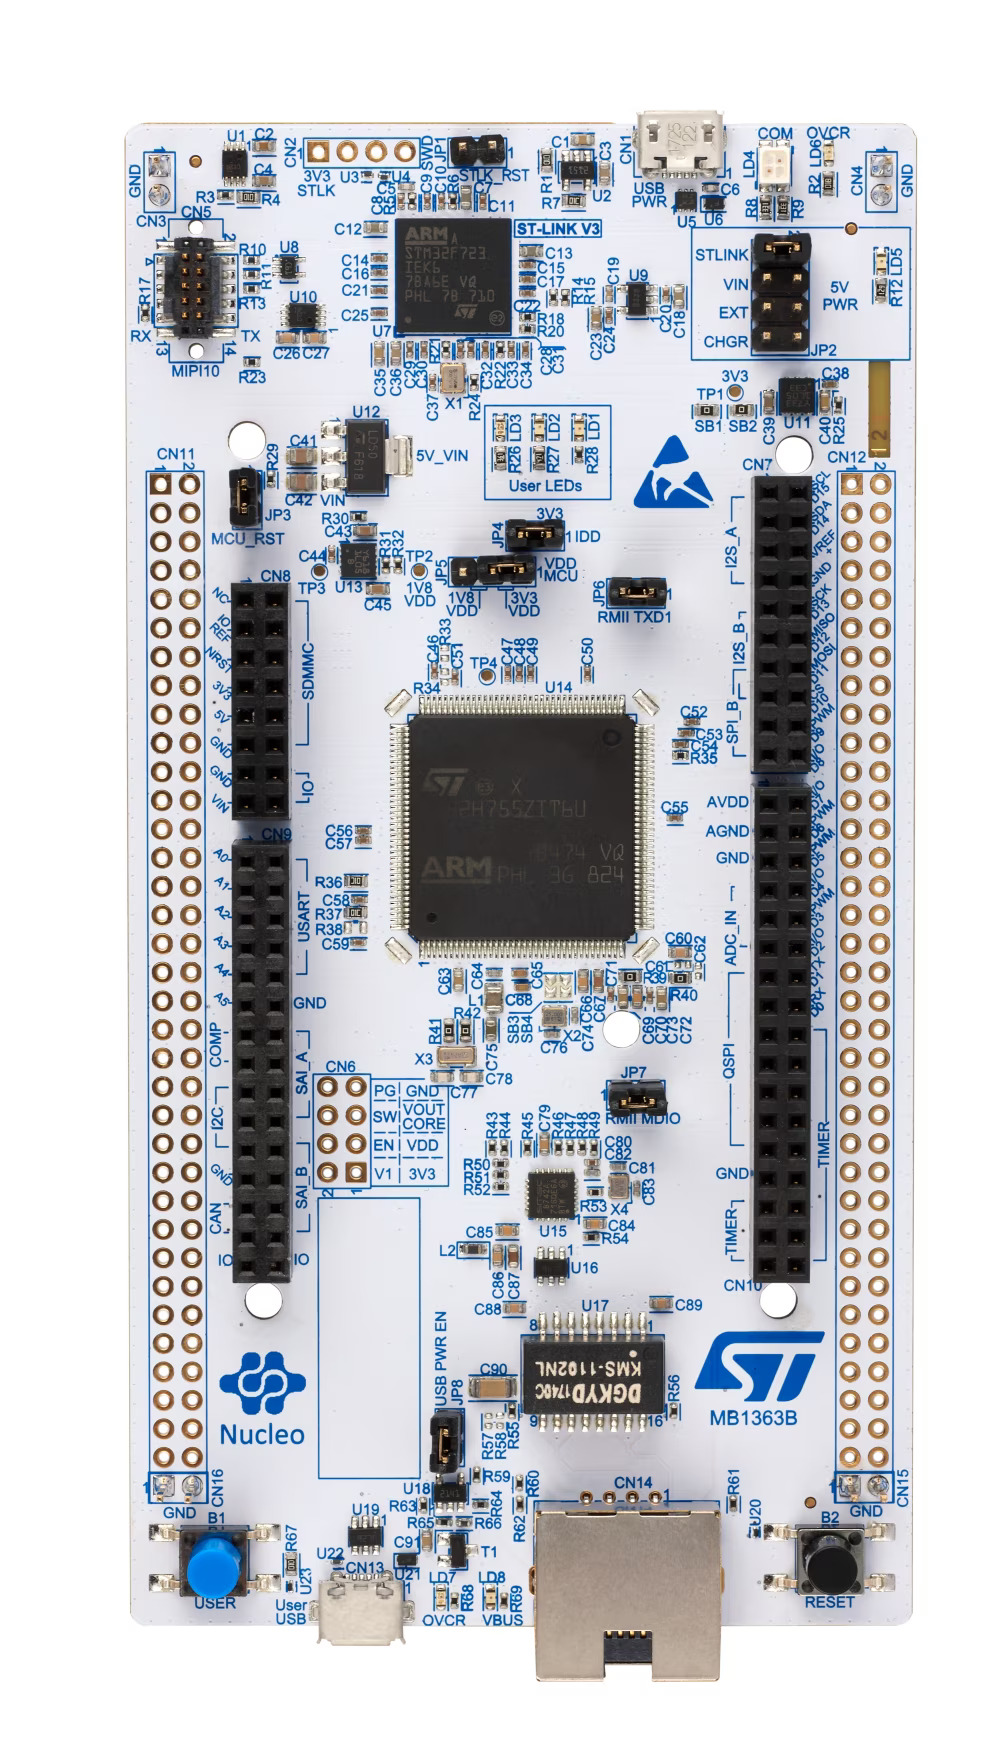
\includegraphics[width = 0.6\textwidth]{images/Immagine_1_relazione__IMMAGINE_STM32H745ZIQ.jpg}
    \caption{NUCLEO STM32-H745ZI-Q}
    \label{fig:etichetta}
\end{figure}
Per un controllo efficiente del Double Propeller Ducted-Fan, è necessaria la conoscenza della cinematica del sistema istante per istante.
L'effettiva conoscenza della cinematica, passa attraverso l'estrapolazione di informazioni da dispositivi capaci di percepire: accelerazione, velocità, posizione e orientamento del sistema interessato.
Per realizzare quest'ultimo interesse, si è optato per l'unità di misura inerziale GY-86, e il sensore di misura della distanza VL53L1X.\\
Nei paragrafi a venire, verranno descritte le caratteristiche dei dispositivi, utilizzate per adempiere all'obiettivo primario.
%fino a qui corretttti gli errori  HMC5983
\section{Modulo GY-86. Unità di misura inerziale}
Al fine di ottenere una struttura compatta, è necessaria la ricerca di un circuito integrato che contiene, sia un accelerometro che un giroscopio, e anche un magnetometro. Per rispettare tale descrizione, si è optato per il modulo GY-86, contenente l'MPU6050 InvenSense e l'HMC5983 Honeywell.
In seguito, un listato delle caratteristiche di funzionamento sfruttate ai fini del progetto.\\\\
\textbf{Caratteristiche principali:}
\begin{itemize}
\item Alimentazione da 3-5 [V].
\item dimensioni : 22 x 17 [mm].
\item Protocollo di comunicazione standard I2C. Supporta una comunicazione I2C fino a\\400 [kHz], "Fast-mode".
\item Un LED di colore verde è utilizzato per segnalare l'avvenuta alimentazione del sistema.
\end{itemize}
Le caratteristiche elencate nel listato precedente, sono comuni a tutti i dispositivi appartenenti al modulo. Pertanto non verranno ripetute nelle descrizioni a seguire. 
    \section{MPU6050 InvenSense}
    L'MPU6050 InvenSense è il primo dispositivo di misura inerziale al mondo a sei assi. Combina un accelerometro a tre assi e un giroscopio a tre assi.\\
    In seguito un elenco delle caratteristiche dell'oggetto che sono state sfruttate nel progetto.\\
    \textbf{Caratteristiche:}
    \begin{itemize}
    \item Alimentazione da 2.375-3.46 [V]. L'alimentazione è gestita dal modulo.
    \item Dimensioni : 4 x 4 x 0.9 [mm].
    \item Possiede un \textit{bus} I2C interamente dedicato all'accettare \textit{input} da una bussola esterna a  tre assi.  
    \item Possiede tre convertitori analogici-digitali per componente (ADCs). La risoluzione di questi è a 16 [bit]. Ottenendo così la digitalizzazione del segnale di uscita del giroscopio e accelerometro.
    \item Tolleranza agli \textit{shock} fino a 10.000 [g]. % convertitore analogico-digital a 16 bit
    \item \textit{Digital Low-Pass Filter} programmabile sia per l'accelerometro che per il giroscopio.
    \end{itemize}
Nel paragrafo seguente verranno descritte le caratteristiche specifiche dell'accelerometro e del giroscopio. Prima però, è opportuna una spiegazione di come questi sensori acquisiscono le misure.
\subsection{Il principio di misura dell'accelerometro e del giroscopio}
\subsubsection{Accelerometro}
L'accelerometro integrato nel dispositivo MPU6050 InvenSense è di tipo capacitivo MEMS, \textit{Micro-Electro-Mechanical Systems}, e consente la misura dell'accelerazione lungo i tre assi cartesiani.\\
Il principio di funzionamento si basa sulla rilevazione delle variazioni di capacità tra microstrutture mobili e fisse realizzate su un substrato di silicio.\\
L'elemento sensibile di ciascun asse è costituito da una massa sospesa, \textit{proof mass}, vincolata da microtravi elastiche ad una cornice ancorata al substrato.
In condizioni di quiete, la massa è in equilibrio e la capacità tra le \textbf{piastre interdigitate*} rimangono simmetriche.\\
Quando il dispositivo è sottoposto ad un'accelerazione lungo uno degli assi sensibili, la massa inerziale si sposta in direzione opposta a quella dell'accelerazione, generando una variazione differenziale 
della capacità tra le piastre.\\
La variazione di capacità viene rilevata da un circuito integrato, che la converte in un segnale elettrico, proporzionale alla velocità applicata.\\
Il segnale analogico prodotto, viene successivamente digitalizzato da un convertitore analogico-digitale a 16 bit, integrato nel chip.
%riprendi controllo da qui 
\subsubsection{Giroscopio}
Il giroscopio integrato nel dispositivo MPU6050 InvenSense è un sensore MEMS di tipo vibrante, \textit{vibrating structure gyroscope}, e consente la misura della velocità angolare lungo i tre assi cartesiani.\\
Il principio di funzionamento si basa sull'effetto Coriolis, che si manifesta quando una massa in moto oscillatorio subisce una rotazione rispetto ad un sistema di riferimento inerziale.\\
All'interno del sensore, ciascun asse dispone di una o più masse vibranti, le quali vengono mantenute in oscillazione a frequenza costante, mediate un circuito di attuazione elettrostatica. Quando il dispositivo ruota attorno ad uno 
degli assi, la massa subisce una forza di Coriolis data da:

\begin{equation}
    \vec{F_c} = 2m(\vec{v}\,\times \,\vec\omega )
\end{equation}
dove \textit{m} è la massa oscillante, $\vec{v}$ è la velocità della massa nella sua traiettoria vibrante, $\vec{w}$ è la velocità angolare del corpo.\\
Questa forza induce uno spostamento trasversale rispetto alla direzione di vibrazione, che viene rilevato attraverso variazioni di capacità tra elettrodi fissi e mobili, similmente a quanto avviene nell'accelerometro.\\
Tali variazioni, proporzionali alla velocità angolare, vengono convertite in un segnale elettrico mediante un circuito di lettura differenziale e successivamente digitalizzate tramite ADC integrato.
\subsection{Accelerometro a tre assi}
L'MPU6050 InvenSense include un accelerometro a tre assi.\\
Il dispositivo utilizza la tecnologia MEMS.\\
Generalmente, l'accelerometro è un dispositivo che fornisce misure sull'accelerazione percepita lungo i tre assi cartesiani.\\
Nel nostro caso, dopo una corretta manipolazione delle informazioni estrapolate, il dato ottenuto rappresenta l'accelerazione in [g], sui tre assi cartesiani.\\
In seguito, un listato descrivente le specifiche caratteristiche, sfruttate ai fini del progetto.\\\\\\\\
\textbf{Caratteristiche specifiche:}
\begin{itemize}
\item L'accelerometro a tre assi fornisce un \textit{output} digitale con \textit{"Full Scale Range"} programmabile dall'utente.\\ Abbiamo quattro diversi \textit{"Full Scale Range"}. Questi sono i \textit{range} dinamici della misura, indicano il massimo valore di accelerazione che può essere misurato lungo i tre assi. Alla fine del paragrafo è stata inserita una tabella che descrive i vari \textit{"Full Scale Range"} dell'accelerometro. 
\item Valore normale di corrente per l'operatività : $500\,[\mu\text{A}]$. Caratteristica gestita dal modulo GY-86.
\item Frequenza di acquisizione delle misure : 1 [kHz].
\item Rilevamento e segnalazione dell'orientamento.
\item Possibilità di effettuare \textit{Self-Test}.
\end{itemize}

\begin{table}[H]
    \centering
    \resizebox{\textwidth}{!}{
    \begin{tabular}{|c|c|c|c|c|}
        \hline 
        \textit{Full Scale Range} & Utilizzo consigliato & Sensibilità & Vantaggi & Svantaggi \\
        \hline
        $\pm 2[g]$ & Applicazioni di alta precisione & Alta : 16384 [LSB]/g & Alta precisione & Rapida saturazione\\
        \hline
        $\pm 4[g]$ & Movimenti Moderati & Media : 8192 [LSB]/g & Buon compromesso & /\\
        \hline
        $\pm 8[g]$ & Attività dinamiche. (Corsa, Robotica mobile) & Bassa : 4096 [LSB]/g & Ampio range & minore precisione\\
        \hline
        $\pm 16[g]$ & Urti, vibrazioni intense, cadute & Molto bassa : 2048 [LSB]/g & Bassa saturazione & precisione scarsa\\
        \hline
    \end{tabular}
    }
    \caption{Full Scale Range Accelerometro}
    \label{tab: tabella}
\end{table}
% peridita
\subsection{Giroscopio a tre assi}
MPU6050 InvenSense include anche un giroscopio a tre assi. Il giroscopio, anch'esso costruito sul disegno della tecnologia MEMS, fornisce misure sulla velocità angolare lungo i tre assi cartesiani.\\
Nel nostro caso, la velocità angolare è espressa in [°/s] (gradi al secondo).\\
A seguire, un elenco descrivente le caratteristiche specifiche, sfruttate ai fini del progetto.\\\\
\textbf{Caratteristiche specifiche:}
\begin{itemize}
\item Il giroscopio a tre assi fornisce un output digitale con \textit{"Full Scale Range"} programmabile dall'utente.\\Anche in questo caso abbiamo quattro diversi \textit{"Full Scale Range"}. Questi, sono i \textit{range} dinamici della misura, indicano il massimo valore di velocità angolare che può essere misurato sui tre assi cartesiani.\\Alla fine del paragrafo, è stata inserita una tabella che descrive i vari \textit{"Full Scale Range"} del giroscopio.
\item Valore normale di corrente per l'operatività : 3.6 [mA].
\item Valore normale di corrente in \textit{standby} : $5\,[\mu\text{A}]$
\item Il sensore fornisce una migliorata stabilità del \textit{bias} e della sensibilità rispetto alla temperatura, che si traduce in una ridotta necessità di calibrazione da parte dell'utente.
\item Buone prestazioni in termini di rumore alle basse frequenze.
\item \textit{"Digital Low-Pass Filter"} programmabile.
\item Frequenza di acquisizione delle misure : 8 [kHz].
\item Possibilità di frazionare la frequenza standard di acquisizione delle misure.
\item Possibilità di effettuare \textit{Self-Test}.
\end{itemize}

\begin{table}[H]
    \centering
    \resizebox{\textwidth}{!}{
    \begin{tabular}{|c|c|c|c|c|}
        \hline 
        \textit{Full Scale Range} & Utilizzo consigliato & Sensibilità & Vantaggi & Svantaggi \\
        \hline
        $\pm 250[°/s]$ & Movimenti lenti e precisi & Alta : 131[LSB]/[°/s] & Alta precisione & Rapida saturazione\\
        \hline
        $\pm 500[°/s]$ & Movimenti moderati(droni a bassa velocità) & Media : 65.5 [LSB]/[°/s] & Buon compromesso & /\\
        \hline
        $\pm 1000[°/s]$ & Movimenti rapidi  & Bassa : 32.8 [LSB]/[°/s] & Ampio range & perdita di dettaglio\\
        \hline
        $\pm 2000[°/s]$ & Rotazioni veloci, urti angolari & Molto bassa : 16.84 [LSB]/[gradi/s] & Bassa saturazione & precisione scarsa\\
        \hline
    \end{tabular}
    }
    \caption{Full Scale Range Giroscopio}
    \label{tab: tabella}
\end{table}
L'obiettivo finale dei test è quello di verificare il corretto funzionamento del sensore e delle librerie sviluppate per gestirlo. La verifica è avvenuta per ogni \textit{Full Scale Range}.

\section{HMC5883L Honeywell}
Lavoro attribuito a Matteo Vitullo

\begin{figure}[H]
    \centering
    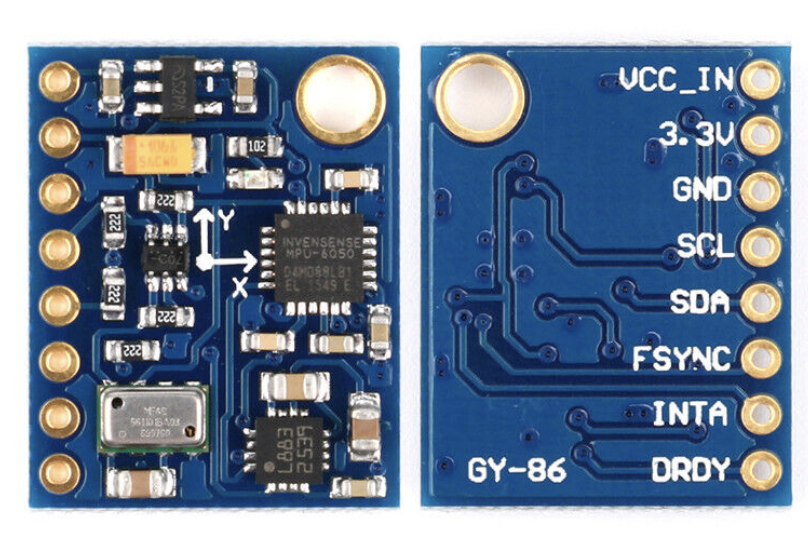
\includegraphics[width = 0.6\textwidth]{images/Immagine_2_modulo_GY_86.png}
    \caption{Modulo GY-86}
    \label{fig:etichetta}
\end{figure}

\section{VL53L1X ST. Sensore Time-of-Flight per la misurazione a lunga distanza}
Per il desiderato comportamento del \textit{Ducted-Fan}, è necessario conoscere la distanza da terra mentre quest'ultimo è in volo. Bisogna, dunque, includere un sensore apposito.\\
Il VL53L1X di STMicroelectronics è pienamente coerente con i requisiti precedentemente espressi.\\
Tuttavia, non si è optato per l'integrazione diretta del sensore della casa STMicroelectronics, si è preferito acquistare il modulo \textit{"iris11a 0J9776"} prodotto da \textit{Pololu}.
Il modulo \textit{breakout} di Pololu, contenente il sensore VL53L1X di STMicroelectronics, è stato scelto per semplificare la fase di configurazione elettronica del sensore.\\
Per comprendere il suo principio di misura, è opportuno dedicare un'intera sezione alla sua descrizione.

\subsection{Il principio di misura \textit{Time-of-Flight}, ToF}
Il principio di misura \textit{Time-of-Flight} si basa sulla determinazione del tempo impiegato da un segnale, generalmente un impulso luminoso nella banda dell'infrarosso, per compiere
un viaggio di andata e ritorno tra un emettitore e un bersaglio riflettente. In particolare, per il nostro dispositivo di misura VL53L1X, la sorgente di emissione luminosa è costituita da
un laser a cavità verticale (VCSEL), che emette brevi impulsi di luce modulata.
Il segnale emesso si propaga nell'ambiente fino ad incontrare un oggetto. Parte della radiazione viene riflessa e raccolta da un rilevatore sensibile alla luce, in genere un array SPAD,
\textit{"Single-Photon Avalanche Diode"}. Questo rilevatore è in grado di registrare l'arrivo anche di singoli fotoni, consentendo una misura estremamente sensibile del tempo di volo.\\
Una volta noto l'intervallo temporale tra l'istante di emissione dell'impulso e quello di ricezione del suo \textit{"eco"}, il calcolo della distanza si ottiene applicando la relazione:
\begin{equation}
    d = \frac{c \cdot \Delta t}{2}
\end{equation}
dove \textit{d} è la distanza dell'oggetto dalla superficie, \textit{c} è la velocità della luce nel vuoto e $\Delta t$ è il tempo di volo misurato. Il fattore 2 al denominatore tiene conto
che il segnale percorre il tragitto due volte, andata e ritorno.\\
I ToF moderni possono utilizzare tecniche avanzate di correlazione temporale o modulazione di fase per migliorare la precisione e la resistenza al rumore ambientale.\\
Nel caso in esame,  il VL53L1X di ST utilizza la tecnologia base ToF o dTof, \textit{"Direct Time-of-Flight"}.\\
\subsection{VL53L1X STMicroelectronics. Caratteristiche}
In seguito, un listato delle principali caratteristiche tecniche del VL53L1X di ST, sfruttante per il progetto.\\
\paragraph{Caratteristiche}
\begin{itemize}
\item Dimensioni : 4.9 x 1.25 x 1.56 [mm]
\item Valore della tensione di alimentazione : 2.6-3.5 [V].
\item Escursione di temperatura per la corretta operatività : da -20 a 85 [°C].
\item Emettitore ad infrarossi di classe [1], di lunghezza d'onda : 940 [nm]. \\Un Laser di classe [1] è un emettitore di onde elettromagnetiche, le cui condizioni operative normali, sono considerate sicure per l'occhio umano e la pelle.
\item Misurazione accurata e veloce. Il dispositivo riesce a misurare distanze fino ai 4 [m] ad una frequenza di acquisizione di 50 [Hz].
\item \textit{Full Field-of-view} standard di 27 [°].
\item \textit{Region-of-interest} (ROI) programmabile. Questa \textit{feature} permette di ridurre il FoV.
\item Presenza di pin di \textit{ShutDown} e di \textit{interrupt}.
\item Sfrutta il protocollo di comunicazione seriale I2C fino a 400[kHz], \textit{Fast-Mode}.
\end{itemize}
Il VL53L1X, come MPU6050, possiede diversi intervalli a piena scala da sfruttare a seconda delle necessità.
\begin{table}[H]
    \centering
    \resizebox{\textwidth}{!}{
    \begin{tabular}{|c|c|c|}
        \hline 
        \textit{Modalità} & Range massimo in codizioni di scarsa luce (approssimato) & Range massimo con luce ambientale \\
        \hline
        \textit{Short} & 136 [cm] & 135 [cm]\\
        \hline
        \textit{Medium} & 290 [cm] & 76 [cm]\\
        \hline
        \textit{Long} & 360 [cm] & 73 [cm]\\
        \hline
    \end{tabular}
    }
    \caption{\textit{Distance mode} del VL53L1X STMicroelectronics.}
    \label{tab: tabella}
\end{table}
\begin{center}
    \footnotesize \textit{Tabella ricavata sotto le seguenti condizioni : \textit{timing budget} = 100 [ms], bersagio bianco, riflettanza : 88\%, luce ambientale : 200 [kcps/SPAD].}
\end{center}

\begin{figure}[H]
    \centering
    \begin{minipage}{0.45\textwidth}
        \centering
        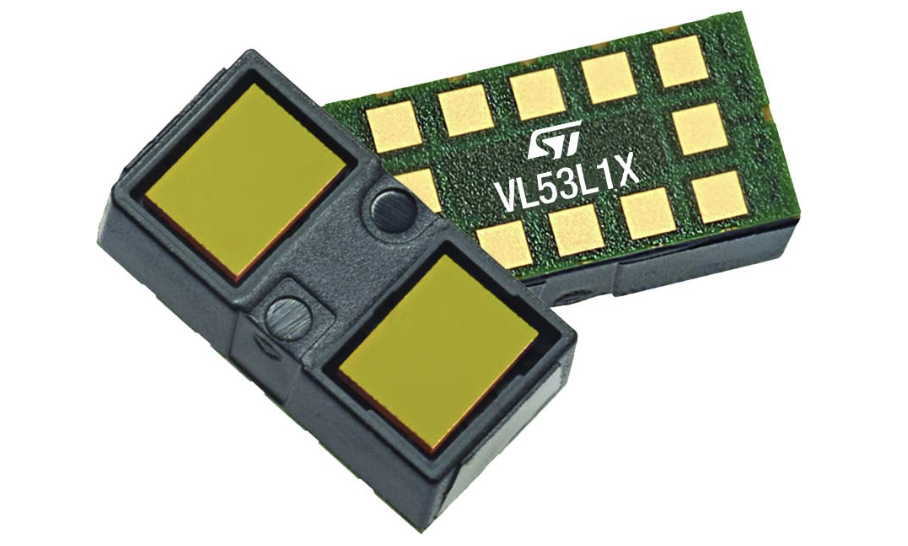
\includegraphics[width=\textwidth]{images/Immagine_3_VL53L1X.png}
        \caption{VL53L1X STMicroelectronics}
        \label{fig:img1}
    \end{minipage}
    \hfill
    \begin{minipage}{0.45\textwidth}
        \centering
        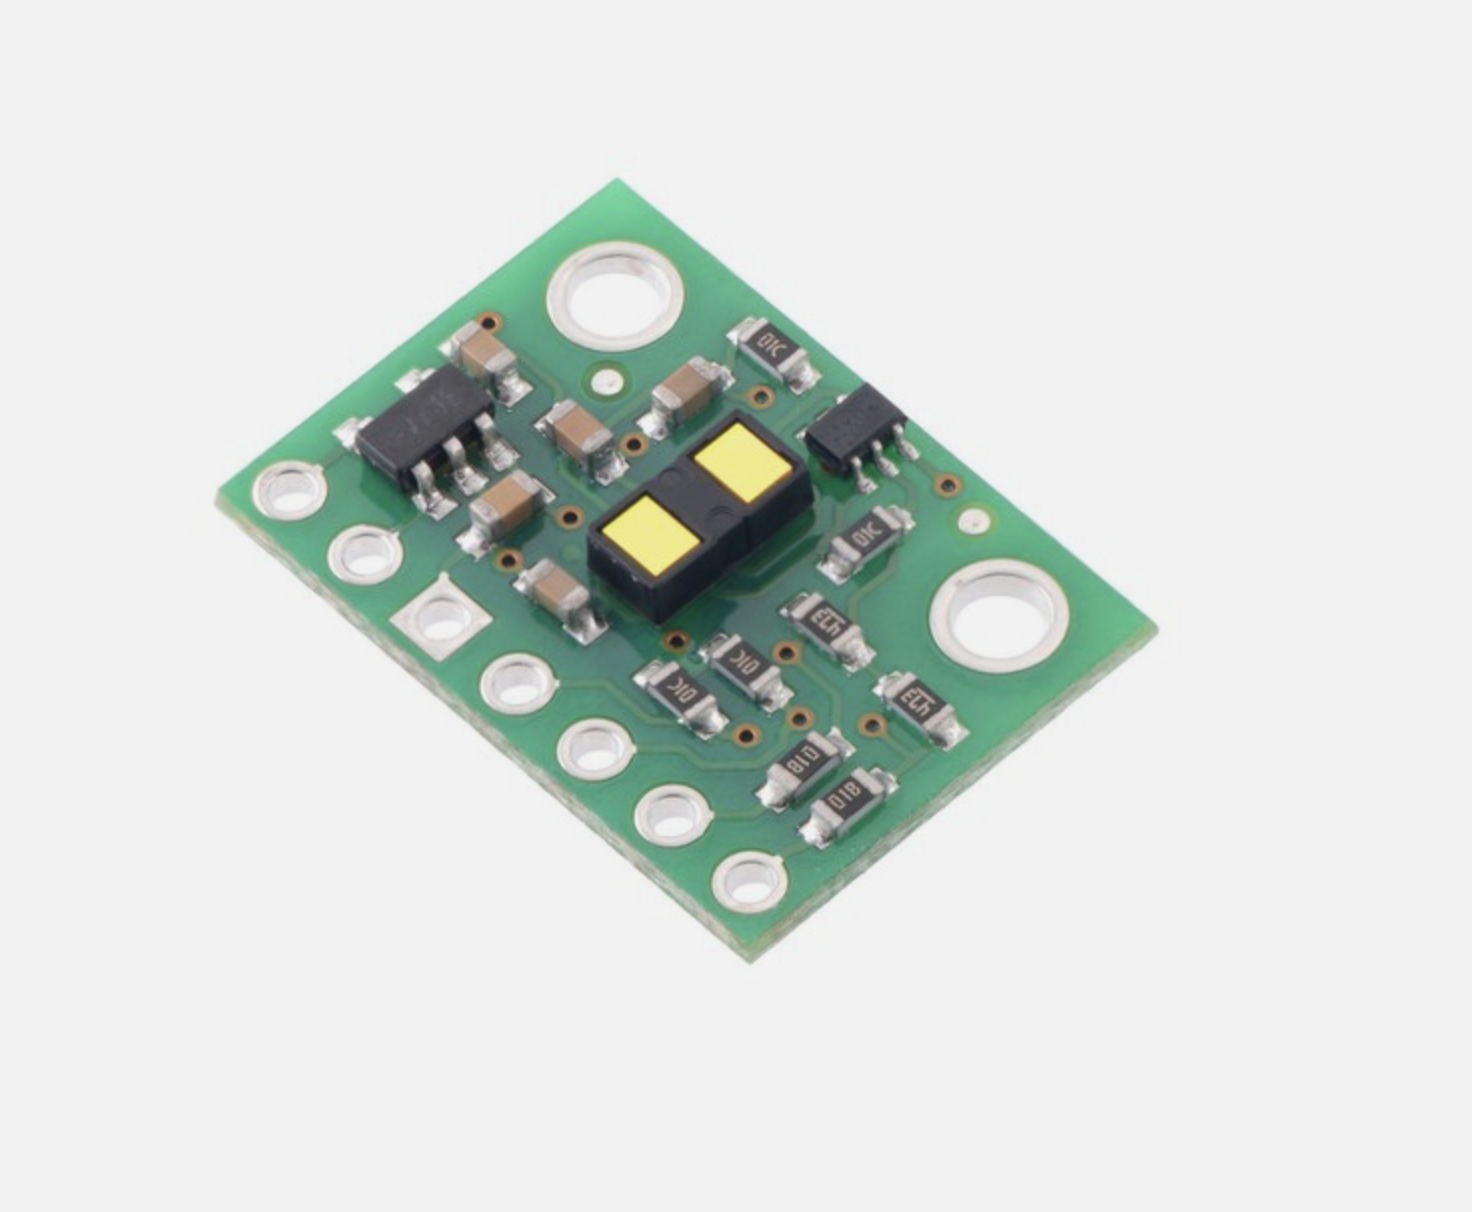
\includegraphics[width=\textwidth]{images/Immagine_4_Pololu.png}
        \caption{Modulo iris11a 0J9776 Pololu contenente il VL53L1X STMicroelectronics}
        \label{fig:img2}
    \end{minipage}
\end{figure}
%qui
\section{Schema dei collegamenti}
Nel sottostante schema è possibile visualizzare lo schema dei collegamenti.
\subsubsection{Modulo GY-86}
Per il GY-86 è stata utilizzata la periferica di comunicazione "I2C1" offerta dalla NUCLEO-H745ZI-Q.
\begin{itemize}
\item VCC del GY-86 collegato al CN8 pin 7   della NUCLEO-H745ZI-Q (3.3[V]).
\item GND del GY-86 collegato al CN8 pin 11  della NUCLEO-H745ZI-Q (GND).
\item SCL del GY-86 collegato al CN10 pin 14 della NUCLEO-H745ZI-Q (PB6).
\item SDA del GY-86 collegato al CN10 pin 16 della NUCLEO-H745ZI-Q. (PB7).
\end{itemize}
\subsubsection{Modulo iris11a 0J9776 Pololu}
Diversamente, per il modulo in questione, è stata utilizzata la periferica di comunicazione "I2C2" offerta dalla NUCELO-H745ZI-Q.
\begin{itemize}
\item VIN del Pololu collegato al CN7 pin 7   della NUCLEO-H745ZI-Q (PB12).
\item GND del Pololu collegato al CN8 pin 13  della NUCLEO-H745ZI-Q (GND).
\item SCL del Pololu collegato al CN10 pin 32 della NUCLEO-H745ZI-Q(PB10).
\item SDA del Pololu collegato al CN10 pin 34 della NUCLEO-H745ZI-Q.(PB11)
\item XSHOUT del Pololu collegato al CN9 pin 29 della NUCLEO-H745ZI-Q (PB14).
\end{itemize}

\begin{figure}[H]
    \centering
    \includegraphics[width=1\textwidth,keepaspectratio]{images/SchemaCollegamentiDrone.drawio.png}
    \caption{Schema dei collegamenti}
    \label{fig:schema}
    \end{figure}

 \chapter{Software}
Al fine di integrare i dispositivi di misura, precedentemente descritti, alla NUCLEO-H745ZI-Q, è stato sviluppato un \textit{firmware} specifico per la gestione della sensoristica.\\
Per quanto riguarda il sensore MPU6050 InvenSense, il firmware di gestione è stato sviluppato interamente da zero. Come detto in precedenza, la scelta è stata necessità più che strategia, dal momento che, per questo dispositivo, non esiste ancora un firmware completo, reperibile dalla rete e adattabile velocemente alla NUCLEO-H745ZI-Q.\\
Diversa è stata l'integrazione del sensore VL53L1X STMicroelectronics. L'azienda produttrice fornisce un firmware ufficiale disponibile sul suo sito internet. Il firmware non è completo quindi è stato modificato per poter operare tramite funzioni HAL ed interfacciarsi correttamente alla NUCLO-H745ZI-Q.\\
Il firmware di gestione dei dispositivi è stato completamente sviluppato utilizzando il linguaggio di programmazione C.\\
Come detto precedentemente l'ambiente di sviluppo integrato (IDE) utilizzato per costruire il \textit{firmware} è stato STCubeIDE fornito da STMicroelectronics. La versione dell'IDE che ha accompagnato tutto lo sviluppo è stata la [1.16.1].\\
Per il \textit{setting} delle periferiche della NUCLEO-H745ZI-Q è stata utilizzata l'interfaccia di programmazione grafica presente in STCubeIDE, STCubeMX.\\
Lo sviluppo è stato completato usando la versione [6.12.1] del STCubeMX.\\
INTRODUZIONE SOFTWARE HMC5883L HONEYWELL.
Nel presente elaborato, i termini procedura e funzione saranno utilizzati come sinonimi, in quanto indicano la medesima entità.
%HMC5983
\section{Diagrammi di flusso}
\subsection{Diagramma di flusso del \textit{firmware} \\dell'MPU6050 InvenSense}
Il seguente \textit{flowchart} descrive la logica di funzionamento del firmware di gestione dell'MPU6050 InvenSense.\\
Nel dettaglio, il diagramma di flusso in analisi presenta graficamente la sequenza di operazioni, decisioni e \textit{loop} del \textit{main flow} del \textit{firmware}.\\
Il diagramma è stato concepito con la finalità di specificare la sequenza di istruzioni da eseguire per la corretta configurazione del dispositivo ed estrazione dell'informazione utile.\\
Le prime due istruzioni ordinano la creazione della struttura di pilotaggio e successivamente la sintesi di un suo puntatore. Punto principale di accesso alla struttura di pilotaggio da parte delle funzioni.\\
Successivamente alle due istruzioni poc'anzi descritte, viene ordinata l'invocazione della  funzione \textit{MPU6050\_InizializzazioneDispositivo}, il cui compito è quello configurare il sensore nella maniera desiderata.\\
Nell' \textit{infinite loop} sono state inserite le funzioni di estrazione e manipolazione dell'informazione legate, rispettivamente, all'accelerometro e al giroscopio.
Tramite un costrutto condizionale e la funzione \textit{MPU6050\_AspettaMisure}, viene gestito il \textit{timing} di estrazione dell'informazione, con il fine di prevedere l'errore di \textit{data overrun}.
Le informazioni estrapolate  poi trasferite alla struttura di pilotaggio da cui sarà possibile effettuarne la lettura.

\begin{figure}[H]
    \centering
    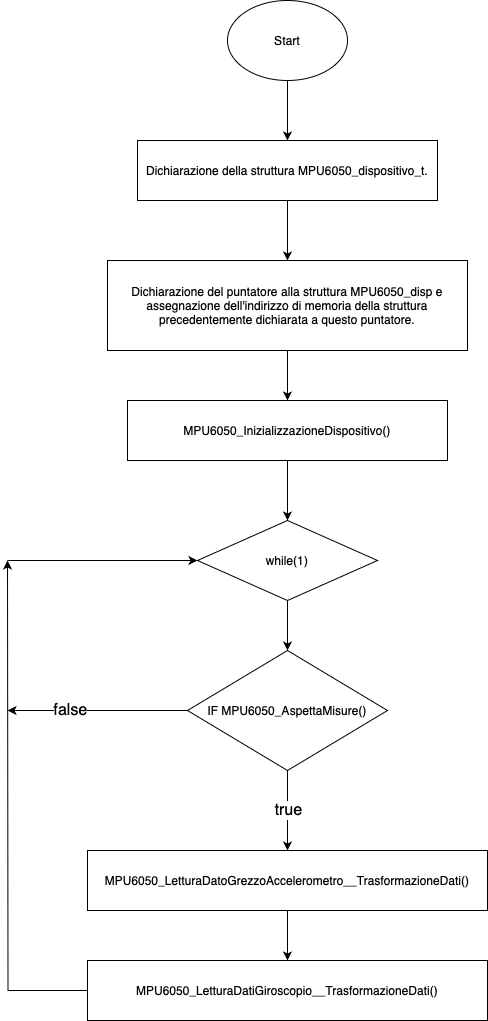
\includegraphics[width=0.5\textwidth,keepaspectratio]{figures copia/Diagramma_di_flusso_GestionMPU6050InvenSense.drawio.png}
    \caption{Diagramma di flusso del \textit{firmware} di gestione dell'MPU6050 InvenSense}
    \label{fig:diagramma 2.1}
\end{figure}

\newpage

\subsection{Diagramma di flusso del \textit{firmware} del VL53L1X STMicroelectronics, STSW-IMG007}
STMicroelectronics fornisce il \textit{firmware} ufficiale di gestione del VL53L1X, l'API \\
STSW-IMG007.\\
La \textit{directory} del STSW-IMG007 contiene un \textit{file} di descrizione dell'API stesso, in questo viene raffigurato il suo \textit{flowchart} di funzionamento.\\
Quest'ultimo, è stato riportato nello scritto, evidenziando però l'utilizzo del \textit{firmware} in\\\textbf{\textit{Driver Polling Mode}}.\\
Il "flusso", inizia con l'invocazione della funzione \textit{VL53L1\_WaitDeviceBooted} che restituirà il \textit{flow} al \textit{main} una volta completato il boot interno del dispositivo.\\
Segue l'istruzione di invocazione, \textit{VL53L1\_DataInit}, procedura che esegue l'inizializzazione dei parametri di \textit{default} interni del sensore, deducendo così una configurazione minima necessaria per iniziare a misurare.\\
Dopo l'inizializzazione primaria, il VL53L1X necessita di una configurazione statica tramite la funzione \textit{VL53L1\_StaticInit}. Questa fase ha il compito di impostare i parametri fondamentali invarianti durante il normale funzionamento del sensore.\\
Durante la \textit{static initialization}, vengono configurate le strutture interne del sensore, tra cui il valore di calibrazione dei tempi, i parametri ottici relativi alla gestione del campo visivo e la gestione delle finestre di misura.\\
Avviene l'impostazione della \textit{distance mode} che determina il comportamento del sensore rispetto alla distanza massima rilevabile e alle condizioni ambientali.\\
Definite le modalità di misura, viene configurato il \textit{Timing Budget}, il tempo massimo che il sensore può dedicare all'esecuzione di una singola misura. Un suo aumento corrisponde all'aumento dell'accuratezza del sensore, a discapito della frequenza di aggiornamento della misura\\
Infine viene definito l'\textit{Inter-Measurement Period}, che stabilisce l'intervallo minimo tra due misure successive.\\
Terminata la fase di configurazione, il \textit{flowchart} comanda l'esecuzione di\\\textit{VL53L1\_StartMeasurement}, impostando il sensore nella modalità di acquisizione autonoma e continua della distanza.
Nell'\textit{infinite loop} il microcontrollore verifica la disponibilità di nuovi dati tramite \textit{VL53L1\_WaitMeasurementDataReady}, se disponibili, il microcontrollore procede alla lettura del risultato di misura invocando la funzione \textit{VL53L1\_GetRangingMeasurementData}.\\
All'estrazione dell'informazione segue il necessario reset della \textit{flag} di \textit{interrupt} interno del sensore mediante \textit{VL53L1\_ClearInterruptAndStartMeasurement}\\
Dopo di che il ciclo ricomincia.


\begin{figure}[H]
    \centering
    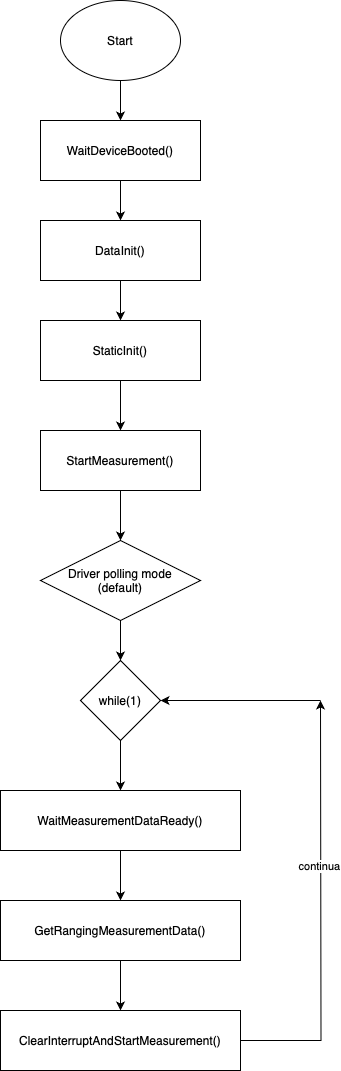
\includegraphics[width=0.4\textwidth,keepaspectratio]{figures copia/VL53L1X_DiagrammaDiFlusso.drawio.png}
    \caption{Diagramma di flusso del \textit{firmware} di gestione del VL51L1X STMicroelectronics}
    \label{fig:diagramma 2.2}
\end{figure}

\subsection{Diagramma di flusso del \textit{firmware} del HMC5883L Honeywell}

\newpage

\section{Descrizione del firmware di gestione dell'MPU6050 InvenSense}
Il \textit{firmware} di gestione dell'MPU6050 InvenSense conta la creazione di quattro file di programmazione.\\
Il \textit{firmware} possiede tre file \textit{header} C, e un unico \textit{source file} in cui sono definite le funzioni principali di gestione del dispositivo di misura.
\subsection{\textit{Header files}}
\subsection{\textit{MPU6050\_register\_map.h}}
Il suddetto file, è stato il primo ad essere sviluppato.\\
Contiene direttive di preprocessore che specificano gli indirizzi, in esadecimale, dei registri dell'MPU6050 InvenSense.\\
Il file è stato creato con il fine di aumentare la leggibilità del codice e semplificarne il successivo sviluppo, soprattutto per tutto ciò che riguarda la comunicazione I2C.\\
Ogni direttiva ha annesso un commento. Questo specifica:
\begin{itemize}
\item Di cosa si occupa il registro indagato e come deve essere programmato.
\item Se il registro interessato è pensato solo per la lettura, per la scrittura o per entrambi.
\item Da quanti bit di memoria è formato il registro.
\end{itemize}
A seguire, un estratto di codice dal file interessato. Il file segue la stessa organizzazione di codice per ogni registro attinto dal progetto.\\
%codice ver 1
\lstinputlisting[language=Cpp, inputencoding=utf8/latin1, firstline=43, lastline=59, caption={Estratto di codice C dal file \textit{MPU6050\_register\_map}}]{codefiles/MPU6050_register_map.h}
Il file contiene solamente direttive di preprocessore quindi non sono stati inclusi altri \textit{header files}.

\subsection{\textit{MPU6050\_platform\_user\_data\_and\_defines.h}}
L'\textit{header file} è stato creato con lo scopo di specificare quali sono le enumerazioni e le strutture dati utilizzate nella gestione dell'MPU6050 InvenSense.\\
Durante lo sviluppo, sono state aggiunte delle direttive di preprocessore il cui fine è aumentare la leggibilità del \textit{core code}.\\
Per una comprensione repentina, il file è stato suddiviso in:
\begin{enumerate}
    \item Enumerazioni.
    \item Strutture dati per la gestione dell'informazione di misura.
    \item Strutture dati aggregate di gestione dell'informazione di misura.
    \item Strutture dati la cui creazione segue il fine di assistenza alle principali funzioni di gestione.
    \item Struttura dati aggregata creata per un pilotaggio intuitivo e semplice\\dell'MPU6050\_InvenSense.
\end{enumerate}

\paragraph{Enumerazioni}
Nella prima sezione, sono disposte le quattro enumerazioni del file.\\
La prima enumerazione, \textit{MPU6050\_valoreDLPF}, è utile nell'impostazione del \textit{"Digital Low-Pass Filter"} del dispositivo.\\
Gli enumeratori definiti al suo interno, hanno una doppia funzione. Aumentare la comprensibilità del codice e contenere
il valore, in esadecimale, che deve essere scritto nel registro CONFIG (registro 26), del dispositivo, per impostare il desiderato \textit{Digital Low-Pass Filter}.\\
A seguire, L'enumerazione.\\
%codice ver 2
\lstinputlisting[language=Cpp, inputencoding=utf8/latin1, firstline=276, lastline=291, caption={Estratto di codice C dal file \textit{MPU6050\_platform\_user\_data\_and\_defines}}]{codefiles/MPU6050_platform_user_data_and_defines.h}
La seconda e la terza enumerazione presente nel file hanno struttura e funzione, analoga alla prima.
Nelle \textit{enum},\\ \textit{MPU6050\_intervalloMisurazioneAccelerometro} e \textit{MPU6050intervalloMisurazioneGiroscopio}, sono specificati i valori del \textit{Full Scale Range} impostabile per l'accelerometro e il giroscopio.\\
Agli enumeratori, inoltre, è stato assegnato il valore, in esadecimale, da scrivere, rispettivamente, nei registri ACCEL\_CONFIG e GYRO\_CONFIG (registro 28,27), per impostare il \textit{Full Scale Range} desiderato.\\
A seguire, le due enumerazioni estratte dal file.
\newpage
%codice ver 3
\lstinputlisting[language=Cpp, inputencoding=utf8/latin1, firstline=294, lastline=322, caption={Estratto di codice C dal file \textit{MPU6050\_platform\_user\_data\_and\_defines}}]{codefiles/MPU6050_platform_user_data_and_defines.h}
L'ultima enumerazione del file è stata creata solo per specificare le modalità di funzionamento dell'MPU6050.\\
A seguire. L'enumerazione.\\
%codice ver 4
\lstinputlisting[language=Cpp, inputencoding=utf8/latin1, firstline=324, lastline=336, caption={Estratto di codice C dal file \textit{MPU6050\_platform\_user\_data\_and\_defines}}]{codefiles/MPU6050_platform_user_data_and_defines.h}

\paragraph{Strutture dati per la gestione dell'informazione di misura}
Nella seconda sezione del file, sono state sviluppate le strutture dati protagoniste nella gestione dell'informazione acquisita dall'accelerometro e dal giroscopio.\\
Per quanto riguarda l'accelerometro, sono state create tre strutture dati.\\
\textbf{MPU6050\_datoGrezzoAccelerometro\_treAssi}, è stata pensata per contenere il segnale grezzo prelevato direttamente dai sei registri: ACCEL\_XOUT\_H, ACCEL\_XOUT\_L,\\ACCEL\_YOUT\_H, ACCEL\_YOUT\_L, ACCEL\_ZOUT\_H, ACCEL\_ZOUT\_L. Questi sono i registri che contengono l'informazione grezza dell'accelerazione lungo i tre assi 
cartesiani.\\  
Ognuno dei registri precedentemente citati presenta memoria ad 8 [bit] nonostante l'informazione finale per ogni asse sia a 16 [bit]. Questo si traduce in una suddivisione  dell'informazione in due parti, la parte alta e la parte bassa. Lo si può, anche, intuire dal nome attribuito a ciascun registro. Se nella parte finale del nome si trova H, questa sta per HIGH e vuol dire che in quel registro troviamo la parte alta dell'informazione. Esatto contrario se troviamo L nella parte finale del nome, questa sta per LOW, e specifica che il registro contiene la parte bassa dell'informazione.\\
Al fine di contenere l'informazione finale è dunque necessario riservare 16 [bit] di memoria, l'effetto ottenuto è una struttura dati composta da tre dati di tipo \textit{uint16\_t}.\\
\textbf{MPU6050\_datoInGAccelerometro\_treAssi} contiene il valore dell'accelerazione in [g] lungo i tre assi cartesiani. Questa è ottenuta dalla lavorazione del dato grezzo estratto da una funzione nel \textit{source file}. I membri della struttura dati sono tutti \textit{float}\\
Infine \textbf{MPU6050\_datoMisuraInternazionaleAccelerometro\_treAssi} è casa del valore dell'accelerazione in [$\frac{m}{s^2}$]. Anche qui troviamo tutti \textit{float}.

\newpage
%codice ver 5
\lstinputlisting[language=Cpp, inputencoding=utf8/latin1, firstline=346, lastline=380, caption={Estratto di codice C dal file \textit{MPU6050\_platform\_user\_data\_and\_defines}}]{codefiles/MPU6050_platform_user_data_and_defines.h}
Per quanto riguarda la sottosezione riservata alle strutture dati del giroscopio, questa è  molto simile a quella dell'accelerometro descritta precedentemente.\\
Sono state sviluppate tre strutture dati.\\
\textbf{MPU6050\_datoGrezzoGiroscopio\_treAssi} è stata concepita per contenere il segnale grezzo prelevato direttamente dai sei registri incaricati. La logica adottata è analoga a quella descritta precedentemente.\\
\textbf{MPU6050\_datoVelocitaaAngolareGiroscopio\_treAssi} è la casa dell'informazione sulla velocità angolare percepita attorno ai tre assi. il dato è ottenuto da una funzione nel \textit{source file} ed è espresso in [$\frac{gradi}{s}$] (gradi al secondo). I membri sono \textit{float}.\\
\textbf{MPU6050\_datoPosizioneAngolareGiroscopio\_treAssi} è stata messa a punto per poter assistere la funzione \textit{MPU6050\_LetturaDatiGiroscopio\_\_TrasformazioneDati}. La struttura dati conta sei membri. Tre di questi sono di tipo \textit{float} e contengono l'informazione di posizione angolare rispetto alla posizione di attivazione del sensore.\\
I restanti, sempre di tipo \textit{float}, contengono il valore della posizione angolare calcolata nell'istante di tempo immediatamente precedente.\\
Questa particolare struttura è il risultato dell'impostazione del calcolo della posizione angolare tramite integrale. Al fine di semplificare la scrittura della funzione, precedentemente citata, si è optato per una modifica diretta della struttura definitrice della posizione angolare.
%codice ver 6
\lstinputlisting[language=Cpp, inputencoding=utf8/latin1, firstline=385, lastline=428, caption={Estratto di codice C dal file \textit{MPU6050\_platform\_user\_data\_and\_defines}}]{codefiles/MPU6050_platform_user_data_and_defines.h}

\paragraph{Strutture dati aggregate}
In questa sezione sono state inserite due strutture dati aggregatrici.\\
Tali strutture sono state adottate al fine di rendere il codice più leggibile e manutenibile.\\
\textbf{MPU6050\_StrutturaDatiAccelerometro\_treAssi} contiene le strutture dati della sezione del file dedicata alle \textit{struct} elementari dell'accelerometro.\\In completa analogia
\textbf{MPU6050\_StrutturaDatiGiroscopi\_treAssi} gestisce la sezione del file dedicata alle strutture del giroscopio.
%codice ver 7
\lstinputlisting[language=Cpp, inputencoding=utf8/latin1, firstline=433, lastline=455, caption={Estratto di codice C dal file \textit{MPU6050\_platform\_user\_data\_and\_defines}}]{codefiles/MPU6050_platform_user_data_and_defines.h}

\paragraph{Struttura dati per l'assistenza a funzioni}
In questa sezione del file è definita un'unica struttura dati.\\
\textbf{assistenza\_MPU6050\_PosizioneAngolareDispositivo} è il risultato di un adattamento. La presenza della struttura ha semplificato lo sviluppo della funzione\\
MPU6050\_LetturaDatiGiroscopio\_\_TrasformazioneDati.
%codice ver 8 
\lstinputlisting[language=Cpp, inputencoding=utf8/latin1, firstline=459, lastline=474, caption={Estratto di codice C dal file \textit{MPU6050\_platform\_user\_data\_and\_defines}}]{codefiles/MPU6050_platform_user_data_and_defines.h}

\paragraph{Struttura dati aggregata per il controllo dell'MPU6050 InvenSense}
L'ultima sezione del file è stata dedicata interamente alla struttura dati aggregatrice principale. Eccetto per la struttura dati definita nella sezione di assistenza delle funzioni, la protagonista aggrega tutte le \textit{struct} trattate in precedenza.\\
Con il fine di semplificare il \textit{main flow} del firmware, i primi due membri della struttura sono tipi di dato definiti nel pacchetto di librerie HAL. Per la corretta compilazione, oltre ad altri file standard,  è stato incluso il file orginale HAL: \textbf{stm32h7xx\_hal.h}.\\
In seguito, un estratto di tutte le inclusioni che troviamo nel file.
%codice ver 9
\lstinputlisting[language=Cpp, inputencoding=utf8/latin1, firstline=9, lastline=13, caption={Estratto di codice C dal file \textit{MPU6050\_platform\_user\_data\_and\_defines} direttive di inclusione}]{codefiles/MPU6050_platform_user_data_and_defines.h}
Il primo membro, \textbf{I2C\_HandleTypeDef perifericaComunicazioneI2C}, gestisce la periferica di comunicazione I2C scelta. La periferica scelta per la comunicazione con il dispositivo dovrà essere programmata usando il \textit{software} di programmazione grafica STCubeMX.
Dopo di ché, STCubeIDE penserà a generare il codice necessario per la sua configurazione. Il risultato di questa operazione si traduce nell'inizializzazione della struttura dati \textbf{I2C\_HandleTypeDef} definita nella HAL. Oltre ad inizializzare automaticamente la struttura dati, viene dichiarata anche una variabile associata
che incarna la periferica scelta. Questa, dovrà essere passata alla struttura dati di pilotaggio dell'MPU6050 InvenSense, per il corretto funzionamento del \textit{core code}.
Analoghe considerazioni per quanto riguarda il secondo membro della struttura, \textbf{UART\_HandleTypeDef perifericaComunicazioneHost}. 
\\Il fine dell'utilizzo della periferica in questione, nasce dalla necessità di verificare il corretto funzionamento del dispositivo.\\
Il protocollo di comunicazione \textbf{UART} è stato accoppiato ad un software esterno, \textit{PuTTy}, per lo scambio di informazioni.\\
La verifica della corretta operatività è stata effettuata tramite \textit{flag} e visualizzazione dati, stampati a video nel terminale offerto dal software di terze parti. Inoltre, questa configurazione è stata sfruttata per poter verificare anche la corretta operatività della sezione del firmware, dedicata alla gestione delle eccezioni.\\
Il terzo membro della struttura contiene l'indirizzo del dispositivo MPU6050, utile al protocollo di comunicazione I2C. Al fine di ottenere la corretta operatività delle funzioni del \textit{core code} si raccomanda l'utilizzo dell'inidirizzo a 8 [bit].\\
In vista di futuri miglioramenti è stato aggiunto anche un membro di tipo \textit{float}, pensato per contenere l'informazione relativa alla temperatura ambientale.\\
A concludere la struttura dati, troviamo un membro incaricato a specificare l'attuale modalità di funzionamento del sensore.\\
Infine, come conclusione del file, è stato definito un nuovo tipo di dato tramite \textit{typedef}. \textbf{MPU6050\_disp} è un puntatore alla struttura dati precedentemente descritta. È stato pensato per essere il principale accesso alla \textit{struct} di pilotaggio. Nel \textit{main flow} dovrà essere definito e inizializzato.\\
In seguito, un estratto raffigurante l'ultima sezione del file.\\\\
%codice ver 10
\lstinputlisting[language=Cpp, inputencoding=utf8/latin1, firstline=480, lastline=505, caption={Estratto di codice C dal file \textit{MPU6050\_platform\_user\_data\_and\_defines} direttive di inclusione}]{codefiles/MPU6050_platform_user_data_and_defines.h}
%inizio  
\subsection{\textit{MPU6050\_platform.h}}
Il file sopra citato è stato pensato e sviluppato al fine di : aumentare l'efficienza di sviluppo, potenziare la leggibilità del codice e disporre di un "navigatore" per spostarsi nel firmware con precisione e all'occorrenza.\\
Il documento di programmazione contiene le dichiarazioni delle funzioni \textbf{core} del firmware, e gli annessi commenti esplicativi del ruolo di queste e del loro funzionamento.\\
Il codice qui sotto presentato offre un primo esempio di organizzazione modulare attraverso l'impiego corretto delle direttive di inclusione, al fine di prevenire eccessive ripetizioni o disorganizzazione nel preprocessore, e favorire una struttura più scalabile e facilmente manutentibile nel tempo.
%codice ver 11
\lstinputlisting[language=Cpp, inputencoding=utf8/latin1, firstline=9, lastline=10, caption={Estratto di codice C dal file \textit{MPU6050\_platform.h} direttive di inclusione}]{codefiles/MPU6050_platform.h}
Il frammento di codice riportato di seguito, è rappresentativo della struttura riccorente del file \textit{header}.

\newpage
%codice ver 12 
\lstinputlisting[language=Cpp, inputencoding=utf8/latin1, firstline=138, lastline=166, caption={Estratto di codice C dal file \textit{MPU6050\_platform.h} esempio con funzione e commento}]{codefiles/MPU6050_platform.h}
\newpage

\subsection{MPU6050\_platform.c. Il \textit{source file} contenente il \textit{core code}.}
\textbf{MPU6050\_platform.c} è stato sviluppato nella considerazione di \textit{file} centrale del firmware. Contiene tutte le definizioni delle funzioni dichiarate nel \textit{file} precedentemente descritto.\\
Le funzioni del \textit{file} sono state create con il fine di soddisfare le richieste del progetto ultimo.\\
Per questioni di navigabilità e leggibilità, anche questo file è stato suddiviso in sezioni.\\
\begin{enumerate}
    \item Direttive di inclusione e variabili \textit{extern}.
    \item Funzione pseudo-contestuale di prima inizializzazione della struttura dati di pilotaggio, MPU6050\_dispositivo\_t.
    \item Verifica della corretta operatività della comunicazione tramite protocollo I2C.
    \item Funzioni di gestione della configurazione dell'MPU6050 InvenSense.
    \item Funzione di \textit{timing}.
    \item Funzioni di lettura e manipolazione delle informazioni.  
\end{enumerate}
È già stato prefissato l'obiettivo futuro di creare una funzione di \textit{Self-Test} per verificare il corretto funzionamento del comparto elettronico del sensore.

\paragraph{Elementi strutturali riccorenti nelle procedure del file}
Lo sviluppo del \textit{source file} è stato guidato dai principi di: semplicità, chiarezza e ripetitività strutturale, con particolare attenzione allo sfruttamento delle risorse messe a disposizione dall'\textbf{\textit{Hardware Abstraction Layer}}.
Al fine di rispettare le linee guida precedentemente elencate, si è scelto di mantenere una struttura ricorrente in tutte le procedure del file.\\
L'enumerazione, \textit{HAL\_StatusTypeDef} è stata scelta come valore di ritorno di ogni funzione del \textit{file}, eccetto per \textit{MPU6050\_PlatformInit} e \textit{MPU6050\_AspettaMisure}.
La ragione della scelta di questo valore di ritorno, nasce dalla necessità di individuare un sistema per la verifica della corretta operatività delle funzioni sviluppate. Il sistema in indagine è stato trovato dando uno sguardo alle librerie dell'HAL.
In queste di fatti, troviamo \textbf{HAL\_StatusTypeDef} che contiene enumeratori indicanti lo stato dell'HAL.\\
L'enumerazione è utilizzata come valore di ritorno della stragrande maggioranza delle funzioni HAL utilizzate in questo progetto. L'integrazione, dunque, di questa enumerazione, anche nelle funzioni sviluppate per la gestione del dispositivo, permette di ottenere 
l'informazione veritiera e concreta sull'operatività delle procedure.\\
A seguite, l'estratto di codice contenente la definizione dell'enumerazione interessata, ottenuta direttamente dal file \textbf{stm32h7xx\_hal\_def.h}.

\newpage
%codice ver 13
\lstinputlisting[language=Cpp, inputencoding=utf8/latin1, firstline=36, lastline=45, caption={Estratto di codice C dal file \textit{stm32h7xx\_hal\_def.h}: definizione di \textit{HAL\_StatusTypeDef}}]{codefiles/stm32h7xx_hal_def.h}

Per una corretta gestione dell'MPU6050 InvenSense, è necessaria la giusta conduzione di scambi di informazione. Al fine di ottenere quest'ultimo risultato, sono state utilizzate procedure definite nell'HAL.\\
Le funzioni HAL, centrali per lo sviluppo di questo \textit{source file} sono:
\begin{itemize}
\item \textbf{\textit{HAL\_UART\_Transmit}}. Gestisce la trasmissione delle informazioni scambiate attraverso protollo di comunicazione UART.
\item \textbf{\textit{HAL\_I2C\_Mem\_Read}}. Utilizza il protocollo di comunicazione I2C per leggere un numero di byte prefissato, dal registro desiderato.
\item \textbf{\textit{HAL\_I2C\_Mem\_Write}}. Funzione inversa di quella precedentemente descritta. Utilizza il protocollo di comunicazione I2C per scrivere un numero di byte prefissato nel registro desiderato.
\end{itemize}
Al fine di una corretta operatività della libreria di gestione, sono state utilizzate altre funzioni del mondo HAL, ma l'utilizzo è limitato alle sole funzioni invocanti e non costituiscono un elemento strutturale ricorrente del \textit{file}.
Per cui verranno analizzate singolarmente in seguito.
La logica adottata per la gestione delle eccezioni e degli errori, ricalca i principi citati poc'anzi. In particolare, ogni funzione è stata sviluppata contenendo il proprio messaggio di errore, che specificherà : la funzione in cui è avvenuta l'eccezione, il tipo di errore e lo stato restituito dalle funzioni HAL invocate nella procedura interessata.\\
La visualizzazione del messaggio di errore avviene per stampa video utilizzando\\\textit{HAL\_UART\_Transmit} e il terminale \textit{PuTTy}.\\
Solo un unico valore di ritorno non verrà mai verificato tramite la procedura precedentemente descritta. Quest'ultimo è il ritorno della funzione \textit{HAL\_UART\_Transmit}, il quale dovrà essere controllato, all'occorenza, usando la funzione di \textit{debugging} offerta da STCubeIDE.
In seguito, la ricorrenza di programmazione circa la gestione delle eccezioni nel \textit{source file}.\\
%codice ver 14
\lstinputlisting[language=Cpp, inputencoding=utf8/latin1, firstline=80, lastline=87, caption={Estratto di codice C dal file \textit{MPU6050\_platform.c}: ricorrenza di programmazione nella gestione delle eccezioni}]{codefiles/MPU6050_platform.c}

La struttura di pilotaggio, come detto nella sottosezione precedente, è stata creata con il fine di semplificare il \textit{main flow} del firmware. La semplicità è situata nelle funzioni di questo file. Qualsiasi procedura del file ha come parametro primo un puntatore alla struttura di interesse.\\
Lo sforzo, dunque, di utilizzo delle funzioni e in generale del firmware, è ridotto grazie a quest'implementazione ricorrente.
Nel seguente frammento, è possibile verificare quanto sia radicata questa ricorrenza, \textit{MPU6050\_disp disp}.
%codice ver 15
\lstinputlisting[language=Cpp, inputencoding=utf8/latin1, firstline=221, lastline=249, caption={Estratto di codice C dal file \textit{MPU6050\_platform.h}: ricorrenza della struttura di pilotaggio nelle procedure}]{codefiles/MPU6050_platform.h}

\paragraph{Direttive di inclusione e variabili \textit{extern}}
%volevo dire che qua si può vedere il risultato delle operazioni effettuate per ottenere una buna organizzazione modulare 
Il risultato dell'organizzazione modulare attraverso il corretto impiego delle direttive di inclusione, è percepibibile in questa prima sezione del file.\\
Al fine di una corretta compilazione del codice, le variabili, rappresentative della comunicazione I2C e UART, sono state dichiarate tramite la direttiva di preprocessore \textit{extern}.
Si è selezionata la modalità descritta nella riga sovrastante per evitare di ridichiarare o ridefinire le due variabili legate alla comunicazione seriale.
In seguito, il frammento di codice raffigurante le inclusioni e le direttive \textit{extern}.
%codice ver 16
\lstinputlisting[language=Cpp, inputencoding=utf8/latin1, firstline=11, lastline=14, caption={Estratto di codice C dal file \textit{MPU6050\_platform.c}: direttive di inclusione e \textit{extern}}]{codefiles/MPU6050_platform.c}



\paragraph{Funzione pseudo-contestuale di prima inizializzazione della struttura dati di pilotaggio. \textit{MPU6050\_PlatformInit}}
La funzione è stata pensata per essere invocata da un'altra procedura.\\
Saltando all'ultima funzione della sezione: \textit{"funzioni di gestione della configurazione\\dell'MPU6050 InvenSense"} troviamo la funzione
\textbf{MPU6050\_InizializzazioneDispositivo}, questa richiama al suo interno tutte le procedure che appartengono alla sezione del file precedente citata e la funzione sotto descrizione.
In questo primo esempio di funzione del \textit{core file}, si può notare quanto la definizione della struttura di pilotaggio principale semplifichi lo sviluppo del firmware.\\
Infatti, questa richiede un solo parametro, un puntatore alla struttura citata.\\ 
L'organizzazione parametrica delle procedure del file seguirà quella poc anzi descritta.\\
La procedura inizializza tutti i membri della struttura di pilotaggio. Le singole inizializzazioni sono state pensate per gestire, all'occorrenza, l'errore legato ad un'incorretta inizializzazione del dispositivo. 
Se per qualche motivo, le funzioni incaricate di comunicare con il dispositivo non dovessero funzionare, in aggiunta ai messaggi di errore di queste, si ha, come strumento di identificazione dell'errore, il controllo dei valori 
assegnati alla struttura di pilotaggio. Le informazioni acquisite dai sensori incorporati non saranno mai pari a zero, dal momento che abbiamo \textit{bias/offset}. Inoltre la modalità di funzionamento del sensore non può essere impostata a [-1].
Tutto quello che è stato esplicato precedentemente vale per tutti i membri della struttura, eccetto i primi tre. Le prime tre assegnazioni hanno un grado di importanza maggiore, dal momento che, definiscono: l'indirizzo del dispositivo MPU6050 come \textit{slave} nella comunicazione I2C, quale periferica di comunicazione, offerta dalla NUCLEO-H745ZI-Q, viene usata per comunicare con il sensore, e la periferica di comunicazione UART con l'\textit{host}.
Di default si assegna la periferica di comunicazione \textbf{hi2c1} e la \textbf{huart3} rispettivamente per il protocollo I2C e UART. Nel caso in cui si avesse la necessità di gestire il dispositivo tramite altre periferiche, bisogna mettere mano alla funzione e modificarne i valori interessati.
A seconda della piattaforma di programmazione utilizzata, è necessario verificare se lo \textit{slave address} del protocollo I2C deve essere a 7[bit] o 8[bit]. Post verifica bisogna modificare il valore dell'indirizzo manualmente. 
In seguito, il frammento rappresentativo del codice.
%codice ver 17
\lstinputlisting[language=Cpp, inputencoding=utf8/latin1, firstline=18, lastline=56, caption={Estratto di codice C dal file \textit{MPU6050\_platform.c}: la funzione \textit{MPU6050\_PlatformInit}}]{codefiles/MPU6050_platform.c}

\paragraph{Verifica della corretta operatività della comunicazione tramite protocollo I2C. \textit{MPU6050\_VerificaComunicazioni}}
Nella sezione interessata, è stata inserita solamente una procedura. \textit{MPU6050\_VerificaComunicazioni} è stata creata con il fine di verificare l'operatività della periferica di comunicazione I2C scelta, oltre che testare lo scambio di informazioni con il dispositivo tramite medesimo protocollo.\\
Nel paragrafo, \textit{Elementi strutturali riccorrenti nelle procedure del file} si specifica che in alcune procedure della libreria, sono state invocate altre funzioni appartenenti al panorama HAL, oltre a quelle comuni nel file.\\
Questo è uno dei casi in esame.\\
La procedura è stata suddivisa in due sezioni.\\
La prima richiede lo stato della periferica di comunicazione I2C scelta, e attende un intervallo di tempo pari a \textit{STANDARD\_TIMEOUT\_MILLISEC} prima di restituire un errore di \textit{time out}. La temporizzazione è gestita manipolando il dato restituito dalla funzione HAL, \textit{HAL\_GetTick}, che utilizza il timer di sistema \textit{SysTickTimer} per scandire correttamente la temporizzazione.\\
La "richiesta di stato" è gestita da un'altra funzione HAL, \textit{HAL\_I2C\_GetState}, che restituisce un dato di tipo enumerato definito sempre nello stesso panorama, \textit{HAL\_I2C\_StateTypeDef}.\\
Se, nei tempi pattuiti, viene restituito il valore \textit{HAL\_I2C\_STATE\_READY}, allora la periferica di comunicazione è pronta per condurre informazioni.\\
Alla seconda sezione, ci si accede solamente se il valore restituito dalla funzione HAL precedente è \textit{HAL\_I2C\_STATE\_READY}. Se questo è il caso, si ha l'invocazione della funzione \textit{HAL\_I2C\_IsDeviceReady}. Quest'ultima verifica, per un certo numero di tentativi prefissabile, se il dispositivo è pronto per lo scambio di informazioni. Se la funzione HAL, non riesce a comunicare con il dispositivo entro il numero di tentativi prefissato o scade il tempo di attesa definito, allora verrà restituito errore, e questo verrà segnalato dal gestore delle eccezioni e lo stato verrà trasmesso come uscita della funzione sviluppata.\\
Se l'operatività corrente è quella prevista, allora si ha la certezza di accuratezza della comunicazione con l'MPU6050 InvenSense.
A seguire, il frammento di codice che riporta la funzione interessata.
%codice ver 18
\lstinputlisting[language=Cpp, inputencoding=utf8/latin1, firstline=59, lastline=113, caption={Estratto di codice C dal file \textit{MPU6050\_platform.c}: la funzione \textit{MPU6050\_VerificaComunicazioni}}]{codefiles/MPU6050_platform.c}

\paragraph{Funzioni configuratrici dell'MPU6050 InvenSense}
La logica adottata dalle procedure sviluppate in questa sezione, nasce dalla necessità di interagire con i registri interni dell'MPU6050 per modificarne i valori.\\
Come discusso nel paragrafo: "Elementi strutturali ricorrenti nelle procedure del file", le procedure hanno un'architettura risonante. Le funzioni di questa sezione adempiono ai loro diversi scopi rispettando \textit{la ricorrenza} più volte citata.
Utilizzano \text{HAL\_I2C\_Mem\_Write} per modificare i valori nei registri interessati e \textit{HAL\_I2C\_Mem\_Read} per leggere i valori di questi.\\
L'architettura di gestione dell'errore è presente come da manuale.
Alla luce del fatto che, la logica di funzionamento è comune a tutte le procedure del file. Verrà puntualizzato solamente il compito che deve essere svolto dalla procedura, e all'occorrenza le "anomalie" rispetto alla \textit{ricorrenza}.
\subparagraph{MPU6050\_ImpostaModFunzionamento}
è la prima funzione della sezione. Quest'ultima imposta la modalità di funzionamento desiderata dell'MPU6050. La procedura, inoltre, gestisce l'errore di impostazione legato ad un valore invalido del parametro: "modFunzionamento".\\
Descrizione delle modalità di funzionamento del sensore.
\begin{itemize}
    \item ACQUISIZIONE\_CONTINUA. Se impostata, il sensore acquisisce le misure dell'accelerazione e della velocità angolare continuamente, rispettando la frequenza di acquisizione dell'accelerometro e del giroscopio. È la modalità di funzionamento di \textit{default}.
    \item SLEEP. Se impostata, l'accelerometro e il giroscopio del sensore vengono disabilitati. Modalità \textit{low-power}.
    \item CYCLE. Se impostata, l'MPU6050 entra periodicamente in modalità di rilevamento, alla frequenza del \textit{Low Power Accelerometer Output Rate}, e acquisisce una misura dall'accelerometro/giroscopio. Tornando poi in \textit{sleep mode} fino al ciclo successivo.
\end{itemize}
La funzione, inoltre, offre la possibilità di effettuare il reset dell'MPU6050 InvenSense. Se opzionato il \textit{Soft-Reset}, i valori nei registri, precedentemente modificati, tornano al loro valore di \textit{default}.\\
Dopo il \textit{Soft Reset}, la procedura si reinvoca, impostando la modalità di funzionamento di \textit{default}, ACQUISIZIONE\_CONTINUA.\\
In seguito, la definizione della funzione presa in esame.
%codice ver 19
\lstinputlisting[language=Cpp, inputencoding=utf8/latin1, firstline=117, lastline=226, caption={Estratto di codice C dal file \textit{MPU6050\_platform.c}: la funzione \textit{MPU6050\_ImpostaModFunzionamento}}]{codefiles/MPU6050_platform.c}
%inizio 
% frammeto
\subparagraph{MPU6050\_ImpostaDLPF.} 
Il compito della procedura sotto analisi, è quello di configurare il \textit{Digital Low-Pass Filter} del dispositivo.\\
Il \textit{Digital Low-Pass Filter} è un filtro digitale interno all'MPU6050 InvenSense, progettato per attenuare il rumore ad alta frequenza nei dati acquisiti da accelerometro e giroscopio.
Se attivo, la frequenza di acquisizione del giroscopio si riduce da 8[kHz] a 1[kHz], mentre quella dell'accelerometro resta invariata ad 1 [kHz].
La procedura modifica il valore della sezione DLPF\_CFG del registro [26]. In seguito, una tabella raffigurante le possibili configurazioni e il loro effetto sulla "prestazione di misura".
\begin{table}[H]
    \centering
    \resizebox{\textwidth}{!}{
    \begin{tabular}{|c|c|c|c|c|c|}
        \hline 
        \textit DLPF\_CFG & Bandwidth ACC (Hz) & Delay ACC (ms) & Bandwidth (Hz) GYRO & Delay GYRO (ms) & Fs (kHz) GYRO\\
        \hline
        $0$ & 260 & 0 & 256 & 0.98 & 8\\
        \hline
        $1$ & 184 & 2.0 & 188 & 1.9 & 1\\
        \hline
        $2$ & 94 & 3.0 & 98 & 2.8 & 1\\
        \hline
        $3$ & 44 & 4.9 & 42 & 4.8 & 1\\
        \hline
        $4$ & 21 & 8.5 & 20 & 8.3 & 1\\
        \hline
        $5$ & 10 & 13.8 & 10 & 13.4 & 1\\
        \hline
        $6$ & 5 & 19.0 & 5 & 18.6 & 1\\
        \hline
    \end{tabular}
    }
    \caption{Le possibili configurazioni opzionabili del \textit{Digital Low-Pass Filter}.}
    \label{tab: tabella}
\end{table}
%codice ver 20
\lstinputlisting[language=Cpp, inputencoding=utf8/latin1, firstline=229, lastline=263, caption={Estratto di codice C dal file \textit{MPU6050\_platform.c}: la funzione \textit{MPU6050\_ImpostaDLPF}}]{codefiles/MPU6050_platform.c}

\subparagraph{MPU6050\_OttieniDLPF.} 
La procedura restituisce il valore del \textit{Digital Low-Pass Filter} attualmente impostato. Nel dettaglio, legge il valore numerico situato nella sezione\\
DLPF\_CFG del registro [26].\\
A seguire, la definizione della funzione.
%codice ver 21
\lstinputlisting[language=Cpp, inputencoding=utf8/latin1, firstline=265, lastline=282, caption={Estratto di codice C dal file \textit{MPU6050\_platform.c}: la funzione \textit{MPU6050\_OttieniDLPF}}]{codefiles/MPU6050_platform.c}

\subparagraph{MPU6050\_ImpostaDivisoreFrequenzaCampionamento.}
Il compito di quest'ultima è quello di impostare il valore del divisore della frequenza di acquisizione del giroscopio.\\
Per rispettare il suo compito, la funzione accede al registro [25] e modifica il valore della sezione SMPLRT\_DIV. La sezione in questione occupa tutta la memoria del registro, 8 [bit], dunque il valore che può essere assegnato al divisore appartiene all'intervallo [0,255].
Con l'impostazione del divisore della frequenza di acquisizione, si hanno tutte le carte in regola per la deduzione della frequenza di acquisizione del giroscopio, che segue la formula:
\begin{equation}
    Fs = \frac{GyroOut}{1 + ValDiv}
\end{equation}
Dove: \textit{Fs} è la frequenza di acquisizione del giroscopio frazionata, \textit{GyroOut} è la frequenza "grezza" di acquisizione del giroscopio, di 8[kHz] se il \textit{DLPF} è disabilitato, 1 [kHz] altrimenti, e \textit{ValDiv} è il valore del divisore della frequenza di acquisizione appena impostato.\\
Ancor più utile nelle applicazioni reali, è la formula inversa in cui si conosce a priori il valore desiderato \textit{Fs} e si vuol dedurre \textit{ValDiv}.
A seguire, la definizione della funzione.
%codice ver 22
\lstinputlisting[language=Cpp, inputencoding=utf8/latin1, firstline=284, lastline=313, caption={Estratto di codice C dal file \textit{MPU6050\_platform.c}: la funzione \textit{MPU6050\_ImpostaDivisoreFrequenzaCampionamento}}]{codefiles/MPU6050_platform.c}

\subparagraph{MPU6050\_OttieniDivisoreFrequenzaCampionamento}
La funzione restituisce il valore del divisore della frequenza di acquisizione del giroscopio. La modalità di funzionamento è la stessa di: "MPU6050\_OttieniDLPF".
La sua definizione.
%codice ver 23
\lstinputlisting[language=Cpp, inputencoding=utf8/latin1, firstline=315, lastline=331, caption={Estratto di codice C dal file \textit{MPU6050\_platform.c}: la funzione \textit{MPU6050\_OttieniDivisoreFrequenzaCampionamento}}]{codefiles/MPU6050_platform.c}

\subparagraph{MPU6050\_ImpostaFullScaleRangeGiroscopio.}
Il nome della "Routine" precede il suo fine, di fatti la funzione imposta il \textit{Full Scale Range} del giroscopio tra quelli disponibili. La funzione, inoltre, gestisce l'errore legato ad un valore non ammesso del \textit{FSR}.\\
Il dettaglio del funzionamento di ogni modalità di misura del giroscopio è stato accennato precedentemente nella tabella (2.2).
Nel seguito, la definizione.
%codice ver 24
\lstinputlisting[language=Cpp, inputencoding=utf8/latin1, firstline=333, lastline=364, caption={Estratto di codice C dal file \textit{MPU6050\_platform.c}: la funzione \textit{MPU6050\_ImpostaFullScaleRangeGiroscopio}}]{codefiles/MPU6050_platform.c}

\subparagraph{MPU6050\_OttieniFullScaleRangeGiroscopio}
Il metodo restituisce il \textit{Full Scale Range} attualmente impostato, del giroscopio. Il valore restituito è un numero che indica l'impostazione associata. Il metodo di funzionamento è analogo alle precedenti \textit{MPU6050\_Ottieni...}\\
Nel seguito, la definizione.
%codice ver 25
\lstinputlisting[language=Cpp, inputencoding=utf8/latin1, firstline=366, lastline=385, caption={Estratto di codice C dal file \textit{MPU6050\_platform.c}: la funzione \textit{MPU6050\_OttieniFullScaleRangeGiroscopio}}]{codefiles/MPU6050_platform.c}
 % operatività pensata
\subparagraph{MPU6050\_ImpostaFullScaleRangeAccelerometro.}
Il fine di questa, è quello di configurare l'intervallo di misura o \textit{Full Scale Range} dell'accelerometro. La tabella (2.1) approfondisce in dettaglio i vari \textit{Full Scale Range} impostabili per l'accelerometro.\\
A seguire, la definizione.
%codice ver 26
\lstinputlisting[language=Cpp, inputencoding=utf8/latin1, firstline=387, lastline=417, caption={Estratto di codice C dal file \textit{MPU6050\_platform.c}: la funzione \textit{MPU6050\_ImpostaFullScaleRangeAccelerometro}}]{codefiles/MPU6050_platform.c}

\subparagraph{MPU6050\_OttieniFullScaleRangeAccelerometro.}
Analogamente ad alcune precedenti funzioni, questa restituisce il \textit{Full Scale Range} attualmente impostato, dell'accelerometro.
Qui sotto, la sua definizione.
%codice ver 27
\lstinputlisting[language=Cpp, inputencoding=utf8/latin1, firstline=419, lastline=436, caption={Estratto di codice C dal file \textit{MPU6050\_platform.c}: la funzione \textit{MPU6050\_OttieniFullScaleRangeAccelerometro}}]{codefiles/MPU6050_platform.c}

\subparagraph{MPU6050\_InizializzazioneDispositivo.}
Il ruolo della procedura, è quello di configurare MPU6050 InvenSense secondo le impostazioni desiderate.\\
In gergo tecnico, la funzione appena citata è una \textit{wrapper function}. La procedura, infatti, invoca tutte le altre funzioni della sezione, aggiungendo al suo record di chiamate anche \textit{MPU6050\_PlatformInit}.\\
I parametri passati alla funzione saranno i parametri delle invocazioni interne.\\
Se solo una delle chiamate interne restituisce un valore diverso da \textit{HAL\_OK}, la funzione si blocca e non completa l'inizializzazione del dispositivo.
Si è optato per l'eliminazione della procedura di gestione dell'errore. Nella presente casistica, di fatti, ogni procedura invocata detiene al suo interno il sistema di gestione dell'errore, dunque, al fine di evitare ridondanze è stata decisa l'omissione del sistema.
\newpage
%codice ver 28
\lstinputlisting[language=Cpp, inputencoding=utf8/latin1, firstline=438, lastline=467, caption={Estratto di codice C dal file \textit{MPU6050\_platform.c}: la funzione \textit{MPU6050\_OttieniFullScaleRangeAccelerometro}}]{codefiles/MPU6050_platform.c}

\paragraph{Funzione di \textit{Timing}. \textit{MPU6050\_AspettaMisure}}
La qui descritta sezione del file conta un'unica funzione. La funzione presenta una struttura di sviluppo diversa dalle altre, di fatti non restituisce il valore di controllo \textit{HAL\_StatusTypeDef} bensì un valore \textit{booleano}. Questo perché,
\textit{MPU6050\_AspettaMisure} verifica la presenza o meno, di nuove misure, acquisite dall'accelerometro e dal gioscopio. A tal fine, il metodo sfrutta una caratteristica hardware dell'MPU6050 InvenSense.
Il bit[0] del registro [58], denominato INT\_STATUS viene automaticamente impostato ad [1] quando una nuova "misura" è disponibile alla lettura.\\
Il metodo dunque, utilizza il connubio tra un \textit{while loop} e un \textit{timer} per gestire la procedura di acquisizione.
Il \textit{flow} del programma rimane nel \textit{while loop} finché non viene letto il valore "true" dal registro oppure finché la procedura non segna il timeout. Per la gestione di quest'ultima, viene utilizzato il timer di sistema SysTickTimer accoppiato alla funzione \textit{HAL\_GetTick}.
Se il \textit{flow} è quello desiderato, la funzione restituisce \textit{"true"} e quindi il via libera alla lettura della misura altrimenti restituisce \textit{"false"}.
La funzione è stata pensata per operare in connubio con una struttura condizionale.
La procedura, inoltre, è stata concepita per evitare l'utilizzo di \textit{timer} nella sincronizzazione tra la velocità di esecuzione del \textit{main.c} e l'acquisizione della misura. In assenza di una corretta temporizzazione, verrebbe acquisita più volte la medesima misura, compromettendo l'efficacia del campionamento e dimunedo l'accuratezza di alcune informazioni ricavate manipolando le misure dirette.
In seguito, il frammento di codice esplicativo dell'operatività prevista per la funzione, e la definizione della funzione stessa.
%codice ver 29
\lstinputlisting[language=Cpp, inputencoding=utf8/latin1, firstline=859, lastline=861, caption={Estratto di codice C dal file \textit{MPU6050\_platform.c}: Dimostrazione dell'uso di \textit{MPU6050\_AspettaMisure}}]{codefiles/MPU6050_platform.c}

\paragraph{Funzioni di lettura e manipolazione delle informazioni}
La sezione ultima del \textit{file} contiene le funzioni di rilevanza maggiore al completamento del progetto.\\
Le procedure qui sviluppate hanno il compito di estrapolare dai registri dell'MPU6050, le misure acquisite dall'accelerometro e dal giroscopio. L'informazione ottenuta verrà poi manipolata dalle medesime con il fine di dedurre misure derivate.
%inizio
\subparagraph{MPU6050\_LetturaDatoGrezzoAccelerometro\_\_TrasformazioneDati e\\ MPU6050\_LetturaDatoGrezzoGiroscopio.}
Le procedure che intitolano il paragrafo, hanno il compito di estrapolare le misure acquisite dall'accelerometro e dal giroscopio.\\Condividono una struttura di sviluppo analoga.\\
Come già scritto in precedenza, i registri che conservano l'informazione di misura dispongono di 8[bit] di memoria, nonostante l'informazione completa sia stata pensata per occupare 16[bit].\\
La risultante di questa particolare configurazione, è l'assegnazione di due registri per la conservazione della misura acquisita lungo un unico asse cartesiano.\\
Nel dettaglio sottostante difatti è possibile notare come sia stata divisa in due registri la misura su un unico asse.
L' "H" nel nome del registro sta ad indicare che in quest'ultimo viene salvata la parte alta dell'informazione [bit8,bit15], mentre la "L" sta ad indicare che il dispositivo conserva in quel registro la parte bassa dell'informazione [bit0,bit7].\\
Ogni asse cartesiano ha questo \textit{"bicromia"}.
\begin{table}[H]
    \centering
    \resizebox{\textwidth}{!}{
    \begin{tabular}{|c|c|c|c|}
        \hline 
        Registri (Hex) Accelerometro &  Nome & Registri (Hex) Giroscopio & Nome\\
        \hline
        3B & ACCEL\_XOUT\_H & 43 & GYRO\_XOUT\_H\\
        \hline
        3C & ACCEL\_XOUT\_L & 44 & GYRO\_XOUT\_L\\
        \hline
        3D & ACCEL\_YOUT\_H & 45 & GYRO\_YOUT\_H\\
        \hline
        3E & ACCEL\_YOUT\_L & 46 & GYRO\_YOUT\_L\\
        \hline
        3F & ACCEL\_ZOUT\_H & 47 & GYRO\_ZOUT\_H\\
        \hline
        40 & ACCEL\_ZOUT\_L & 48 & GYRO\_ZOUT\_L\\
        \hline
    \end{tabular}
    }
    \caption{Dettaglio sull'adiacenza dei registri contenenti l'informazione}
    \label{tab: tabella}
\end{table}
Per l'acquisizione delle informazioni interessate, viene effettuata una lettura sequenziale di 6[byte], sfruttando l'adiacenza dei registri interni del dispositivo.
Nello specifico, le procedure utilizzano un'unica invocazione di \textit{HAL\_I2C\_Mem\_Read}, comandando la lettura di 6[byte] partendo dal registro indicizzato con il valore in esadecimale più piccolo. L'adiacenza poc'anzi citata, viene adottata per compiere un'unica operazione di lettura, aumentando l'efficienza del codice.\\
Le funzioni sono state sviluppate in modo che i 6[byte] di memoria letti dai registri, vengano salvati in un \textit{array} composto da sei celle, specializzate nel contenimento di dati \textit{uint8\_t}.
Supponendo di effettuare l'operazione di lettura sequenziale dai registri contenenti le misure dell'accelerometro, la prima cella dell'\textit{array} conterrebbe la parte alta della misura dell'accelerazione percepita lungo l'asse delle ascisse, mentre la seconda, la parte bassa per lo stesso asse, e così via per i restanti.
Si può dire, dunque, che avviene il trasferimento della rigorosa struttura dei registri, all'\textit{array} sovra citato.\\
Per il completamento dell'informazione grezza, viene effettuata l'assegnazione di questa alle variabili della struttura di pilotaggio, mediante un'operazione OR bit per bit con \textit{cast} finale (\textit{int16\_t}), con il fine di generare il dato completo a 16[bit].\\
Per ottenere la misura ultima, bisogna manipolare il segnale grezzo con una metodologia dipendente dal \textit{Full Scale Range} attualmente impostato. Viene, quindi, richiamata la procedura di restituzione del \textit{FSR} a seconda del componente interessato.\\
Il costrutto \textit{switch-case} indirizzerà il \textit{flow} del programma alla parte di codice che gestisce la manipolazione della misura per quel determinato valore di \textit{FSR}, sia per il giroscopio che per l'accelerometro. Le singole sezioni del costrutto sono pensate per assegnare l'informazione ultima alle variabili specializzate della struttura di pilotaggio.
L'assegnazione è, il risultato del rapporto tra il segnale grezzo e la sensibilità specifica di quel \textit{FSR}.\\
Le funzioni intitolanti il paragrafo, nonostante l'analogia strutturale hanno alcune diversità legate alla deduzione dell'informazione derivata.
%inizio
\subparagraph{Analisi sulla manipolazione dei dati di\\MPU6050\_LetturaDatoGrezzoAccelerometro\_\_TrasformazioneDati.}
La procedura in questione, interagisce con l'accelerometro.\\
All'estrapolazione dell'informazione segue la sua manipolazione. Come detto in precedenza, il segnale grezzo, estratto dai registri del dispositivo, dovrà essere diviso per il valore di sensibilità, dipendente dal \textit{Full Scale Range} dell'accelerometro attualmente impostato.\\
Il risultato di questa operazione, è il valore di accelerazione percepito lungo i tre assi, espresso in [g]. La funzione elabora ulteriormente questo dato per poter ottenere l'accelerazione espressa in [$\frac{m}{s^2}$]. L'elaborazione in questione è banale, difatti viene solamente effettuata la trasformazione da [g] a [$\frac{m}{s^2}$], moltiplicando la prima informazione per [9,81].
Nel seguio, è stata riportata la definizione della funzione interessata.
%codice ver 30
\lstinputlisting[language=Cpp, inputencoding=utf8/latin1, firstline=501, lastline=594, caption={Estratto di codice C dal file \textit{MPU6050\_platform.c}: la funzione \textit{MPU6050\_LetturaDatiAccelerometro\_\_TrasformazioneDati}}]{codefiles/MPU6050_platform.c}

\subparagraph{Funzioni di lettura e manipolazione dell'informazione interagenti con il giroscopio}
\textit{MPU6050\_LetturaDatoGrezzoAccelerometro\_\_TrasformazioneDati} ha il compito di estrapolare l'informazione e manipolarla. Diverso è l'approccio adottato per la gestione dell'informazione acquisita dal giroscopio.

La differenza tra la gestione dell'informazione dell'accelerometro e quella del giroscopio è sia strutturale che concettuale. La diversità degli approcci nasce in primis dalle richieste progettuali.\\
Il progetto richiede dall'accelerometro solo la misura dell'accelerazione lungo i tre assi cartesiani. La complessità di soddisfacimento della richiesta è minima, dato che l'accelerometro è stato progettato proprio per fornire tale informazione.
La richiesta di informazioni dal progetto al giroscopio è particolarmente più stringente di quella analizzata in precedenza. La richiesta non si ferma soltanto alla misura della velocità angolare ma anche alla determinazione del verso di rotazione e della posizione angolare.\\
Aumentando la complessità legata alla gestione dell'informazione.
Con il fine di soddisfare tali richieste, si è optato per lo sviluppo di due funzioni per la gestione dell'informazione.

\subparagraph{MPU6050\_LetturaDatoGrezzoGiroscopio}
La funzione intitolante è una \textit{helper function}, vale a dire che è stata concepita come supporto nell'esecuzione di un'altra funzione.\\
\textit{MPU6050\_LetturaDatiGiroscopio\_\_TrasformazioneDati} nel nostro caso.\\
La procedura ha il compito di estrapolare l'informazione della velocità angolare dal giroscopio. La metodologia di estrazione è stata descritta precedentemente. 
La prima manipolazione dell'informazione corrisponde al rapporto tra il segnale grezzo acquisito dai registri e la sensibilità, dipendente sempre dal \textit{Full Scale Range}.\\
L'MPU6050 InvenSense offre, inoltre, la possibilità di individuare il senso di rotazione.\\
Nello specifico, quest'ultima informazione non viene identificata esprimendola attraverso \textit{segno}. Per meglio dire, il senso orario non è individuato mediante segno negativo associato all'informazione della velocità angolare.\\
Il sensore offre l'informazione della velocità di rotazione, occupando tutto l'intervallo d'escursione del \textit{Full Scale Range} attualmente impostato. In altre parole, supponendo la configurazione con \textit{FSR = $\pm250[\frac{gradi}{s}]$}, la misura della velocità angolare in uscita apparterrebbe all'intervallo [0,500].
Questo poiché, il sensore, attribuisce ad una metà dell'intervallo di escursione, un senso di rotazione, e all'altra metà, la rimanente direzione. Tornando all'assunzione precedente, se nella misura si individuassero valori appartenenti a [0,250], allora questi esprimerebbero la velocità di rotazione in direzione antioraria. 
Nel caso in cui si trovassero della misure appartenenti a [500,250] queste esprimerebbero la velocità di rotazione nella restante direzione.\\
Medesime conclusioni valgono per tutti i \textit{Full Scale Range} del dispositivo.\\
La funzione è stata sviluppata per elaborare questa metodologia di espressione, fornendo l'informazione del senso di rotazione mediate segno. La manipolazione avviene per costrutto condizionale ed, ovviamente, per ogni \textit{Full Scale Range}.
A seguire, la sua definizione.
%codice ver 31
\lstinputlisting[language=Cpp, inputencoding=utf8/latin1, firstline=710, lastline=851, caption={Estratto di codice C dal file \textit{MPU6050\_platform.c}: la funzione \textit{MPU6050\_LetturaDatoGrezzoGiroscopio}}]{codefiles/MPU6050_platform.c}
%  primale
\subparagraph{MPU6050\_LetturaDatiGiroscopio\_\_TrasformazioneDati}
La procedura in questione, ha il compito di stimare la posizione angolare del dispositivo.\\
La stima basa la sua deduzione sulla velocità angolare del dispositivo. 
Al fine della deduzione, la velocità di rotazione del dispositivo deve essere integrata nel tempo.
Trattandosi di dispositivi digitali, necessaria è la teoria legata all'integrazione discreta.
Per questa prima versione, si è optato per la formula di integrazione discreta del trapezio. La sua forma compatta :
\begin{equation}
    \int_{a}^{b} f(t)\, dt \approx \frac{h}{2} \left( f(k_0) + 2 \sum_{i=1}^{n-1} f(k_i) + f(k_n) \right)
\end{equation}
in cui: \textit{k} identifica il tempo discreto, $h=\frac{b-a}{n}$ e $f(k_i)$ sono i valori discreti di velocità angolare.\\
Con il fine di adattare la formula al codice, è stata utilizzata la seguente :
\begin{equation}
    \approx \frac{\delta t}{2} \left(f(t_i)+f(t_{i+1})\right)  \quad \delta t = t_{i+1} - t_i
\end{equation} 

facilemente ricavabile dalla forma compatta ponendo $n=1$.\\
Considerando $\delta t$ pari al tempo di acquisizione dell'informazione da parte del giroscopio, possiamo determinare il valore della posizione angolare del dispositivo.\\
In pseudocodice.
\begin{lstlisting}[language = Cpp]
    while(...){
        posizione_angolare_attuale = valore_integrale + (1/2)*deltat*( vel_ang_ist_prec + vel_ang_ist_att);
        valore_integrale = posizione_angolare_attuale;
        }
\end{lstlisting}
Con il fine di adottare la logica precedentemente esposta, è stato necessario lo sviluppo di codice utile all'individuazione della frequenza di acquisizione del giroscopio.\\
Avvengono le invocazioni delle funzioni \textit{MPU6050\_OttieniDivisoreFrequenzaCampionamento} e \textit{MPU6050\_OttieniDLPF}.\\
La deduzione della frequenza di campionamento del giroscopio, segue la formula citata nel patagrafo \textit{MPU6050\_ImpostaDivisoreFrequenzaCampionamento}. %magati mettici il numero alla formula così da tener traccia di queste
Un costrutto condizionale distingue tra le due frequenze di lavoro "grezzo" del giroscopio, \textit{DLPF on} e \textit{DLPF off}, rispettivamente $1 [kHz]$ e $8 [kHz]$.
Una volta determinata la frequenza di acquisizione propria del giroscopio, la procedura determina il $\delta t$, l'intervallo di tempo tra un'acquisizione e l'altra, calcolando l'inverso della frequenza di acquisizione del giroscopio.
Seguendo la formula del trapezio applicata al singolo intervallo, viene invocata la funzione \textit{MPU6050\_AspettaMisure} per gestire il \textit{timing} tra un'acquisizione e l'altra. Acquisendo così, il valore della velocità angolare nell'istante di tempo precedente, e quello nell'istante di tempo puntuale.\\
L'intervallo di appartenenza scelto per la posizione angolare è [0,360][°]. Per la gestione dell'eccedenza rispetto a tale intervallo si è scelto uno sviluppo basato sul costrutto condizionale.
A seguire il codice.
%codice ver 32
\lstinputlisting[language=Cpp, inputencoding=utf8/latin1, firstline=596, lastline=708, caption={Estratto di codice C dal file \textit{MPU6050\_platform.c}: la funzione \textit{MPU6050\_LetturaDatoGrezzoGiroscopio}}]{codefiles/MPU6050_platform.c}
La procedura qui descritta è stata concepita come protagonista per l'acquisizione di informazioni dal giroscopio. La presenza nel \textit{main flow} è consigliata.

%%%%%%%%%%%%%%%%%% DESCRIZIONE DEL VL53L1X %%%%%%%%%%%%%%%%%

\section{Descrizione del firmware di gestione del VL53L1X STMicroelectronics. STSW-IMG007 FULL API}
STMicroelectronics, produttore del VL53L1X, fornisce il \textit{firmware} ufficiale di gestione del dispositivo, sviluppato mediante linguaggio C. Il \textit{firmware} di interesse è chiamato\\\textbf{STSW-IMG007 FULL API}\\
Con il fine di risparmiare tempo per il compimento della \textit{task}, è stata preferita l'implementazione del firmware ufficiale piuttosto che lo sviluppo autonomo.
Il \textit{firmware} di STMicroelectronics è \textbf{multi piattaforma}, vale a dire che è stato concepito per operare, oltre che su STCubeIDE, anche su altri ambienti di sviluppo.
In virtù di ciò, è necessario operare un'adattamento all'ambiente di sviluppo utilizzato.\\
Gli sviluppatori del firmware hanno ridotto il lavoro necessario all'adattamento, difatti, per raggiungere tal fine è sufficiente metter mano alla cartella \textit{platform}. Per lo scopo primario è risultata sufficiente la modifica di \textit{vl53l1\_platform.c}.\\
Al fine di garantire la corretta operatività del \textit{firmware}, si è optato per un adattamento tramite funzioni HAL, del tipo descritte in precedenza.\\
l'adozione delle strutture software HAL è consequenziale all'impiego di tipologie di dato, strutture, introdotte nei paragrafi precedenti.
 
\subsection{Il \textit{source file} di adattamento. \textit{vl53l1\_platform.c}}
Le procedure, la cui definizione è a carico del consumatore finale, sono state individuate durante l'esecuzione del codice. Le segnalazioni di errore di STCubeIDE sono state utili alla localizzazione di tali indefinite funzioni.
Lo studio del contesto delle procedure da definire, è stato la chiave del corretto adattamento.
Anche in questo caso, con il fine di migliorare la leggibilità del codice, si è optato per la divisione del file in sezioni. Nel dettaglio, \textit{vl53l1\_platform.c} è stato diviso in due sezioni.
La prima corrispondente al firmware ufficiale, la seconda legata alla definizione delle funzioni di adattamento.\\
In questo scritto non verranno menzionati altri file al di fuori di \textit{vl53l1\_platform.c}, inoltre non verranno discusse procedure che non sono state sviluppate al fine dell'adattamento.
La comunicazione I2C con il dispositivo è gestita dalla periferica I2C2 della NUCLEO-H745ZI-Q.\\
Al fine di verificare la corretta operatività delle funzioni implementate, come nel caso del modulo GY-86, si è optato per l'utilizzo di un terminale per la stampa video di informazioni. Il terminale in questione, è fornito dal software esterno \textit{PuTTy}, precedentemente menzionato.\\
Per comunicare le informazioni esprimenti l'operatività delle implementazioni, \textit{PuTTy} utilizza il protocollo di comunicazione seriale UART. In analogia con la metodologia di gestione dell'MPU6050 InvenSense, per la comunicazione in questione è stata scelta la periferica di comunicazione USART3 della NUCLEO-H745ZIQ.
Entrambe le periferiche di comunicazione vengono gestite dall'HAL, tramite le strutture \textit{I2C\_HandleTypeDef} e \textit{UART\_HandleTypeDef}.\\
Con il fine di includere la libreria di funzioni HAl, è stata necessaria l'inclusione di\\\textit{stm32h7xx\_hal.h} in \textit{vl53l1\_platform.c}.\\
Anche in questo caso per evitare problemi di compilazione, nel \textit{file vl53l1\_platform.c} sono state ri-definite le variabili di controllo di tali periferiche con direttiva "extern".\\
Ri-dichiarazione delle variabili. In aggiunta, le direttive di inclusione.

\begin{lstlisting}[language = Cpp, caption={\textit{path} delle direttive di inclusione di \textit{vl53l1\_platform.c}, in aggiunta la ridefinizione delle variabili di gestione della comunicazione}]

    //direttive di inclusione aggiunte
   #include "stdio.h"
   #include "stdint.h"
   #include "stm32h7xx_hal.h"
    
    //direttive di inclusione originali
    #include "vl53l1_platform.h"
    #include "vl53l1_platform_log.h"

    //direttive extern
    extern I2C_HandleTypeDef hi2c2;
    extern UART_HandleTypeDef huart3;

\end{lstlisting}

Il \textit{firmware}, per ragioni deducibili, non gestisce l'errore mediante implementazione HAL. Possiede invece un sistema di gestione dell'errore originale.\\
La struttura utilizzata dal \textit{firmware} per la segnalazione dell'insorgenza di eccezioni, è un'\textit{alias} di tipo.
\textit{VL53L1\_Error} è il tipo di dato utilizzato dal \textit{firmware} allo scopo. Di conseguenza tutte le funzioni di \textit{vl53l1\_platform.c} restituiscono il tipo di dato citato in precedenza.\\
Questo sistema di gestione dell'errore, è stato utilizzato durante lo sviluppo, per la verifica del corretto funzionamento delle implementazioni.\\
In alcune definizioni, è stata forzata la "collaborazione", tra la struttura di gestione delle eccezioni della libreria HAL e quella presente nel \textit{firmware} sotto analisi.
%  poc anzi
\begin{lstlisting}[language=Cpp, caption={Dettaglio sulla struttura di gestione delle eccezioni presente in \textit{vl53l1\_error\_codes.h} da notare, il cast a dato VL53L1\_Error nelle direttive \textit{define}}]
    
    typedef int8_t VL53L1_Error;

#define VL53L1_ERROR_NONE                              ((VL53L1_Error)  0)
#define VL53L1_ERROR_CALIBRATION_WARNING               ((VL53L1_Error) - 1)
	/*!< Warning invalid calibration data may be in used
		\a  VL53L1_InitData()
		\a VL53L1_GetOffsetCalibrationData
		\a VL53L1_SetOffsetCalibrationData */
#define VL53L1_ERROR_MIN_CLIPPED                       ((VL53L1_Error) - 2)
	/*!< Warning parameter passed was clipped to min before to be applied */

define VL53L1_ERROR_UNDEFINED                         ((VL53L1_Error) - 3)

#define VL53L1_ERROR_INVALID_PARAMS                    ((VL53L1_Error) - 4)
	/*!< Parameter passed is invalid or out of range */
#define VL53L1_ERROR_NOT_SUPPORTED                     ((VL53L1_Error) - 5)
	/*!< Function is not supported in current mode or configuration */
#define VL53L1_ERROR_RANGE_ERROR                       ((VL53L1_Error) - 6)
	/*!< Device report a ranging error interrupt status */
#define VL53L1_ERROR_TIME_OUT                          ((VL53L1_Error) - 7)
	/*!< Aborted due to time out */
#define VL53L1_ERROR_MODE_NOT_SUPPORTED                ((VL53L1_Error) - 8)
	/*!< Asked mode is not supported by the device */
#define VL53L1_ERROR_BUFFER_TOO_SMALL                  ((VL53L1_Error) - 9)
	/*!< ... */
#define VL53L1_ERROR_COMMS_BUFFER_TOO_SMALL            ((VL53L1_Error) - 10)

\end{lstlisting}
A seguire, la descrizione delle procedure implementate con il fine di ottenere il corretto interfacciamento con l'\textit{MCU} di interesse.


\paragraph{RANGING\_SENSOR\_COMMS\_Init\_CCI}
Nell'analisi della funzione\\\textit{VL53L1\_CommsInitialise}, il cui compito, è quello di inizializzare le periferiche di comunicazione in utilizzo, è stata individuata la prima procedura utile all'adattamento.\\
\textit{RANGING\_SENSOR\_COMMS\_Init\_CCI} è invocata dalla precedente procedura, con lo scopo di ottenere la verifica della corretta operatività della periferica di comunicazione in uso.
Per lo sviluppo della definizione della funzione è stata necessaria l'integrazione dell'HAL.\\
La componente HAL utilizzata per l'adattamento è \textit{HAL\_I2C\_GetState}, già descritta nella sezione dedicata alla descrizione del \textit{firmware} di gestione dell'MPU6050.
La funzione restituisce il valore, a sua volta, viene restituito da \textit{HAL\_I2C\_GetState}.\\
La procedura invocatrice \textit{VL53L1\_CommsInitialise}, è stata modificata per adattarsi al valore di restituzione di \textit{RANGING\_SENSOR\_COMMS\_Init\_CCI}.\\
Per ottenere la corretta operatività della funzione invocatrice è, dunque, necessaria la restituzione di \textit{HAL\_I2C\_STATE\_READY} da parte di \textit{RANGING\_SENSOR\_COMMS\_Init\_CCI}.
Se dovesse verificarsi la situazione poc'anzi descritta, \textit{VL53L1\_CommsInitialise} risulterebbe invocata con successo, altrimenti verrà gestita l'eccezione tramite restituzione di un parametro \textit{VL53L1\_Error}.
A seguire la definizione della funzione, e un breve frammento specificante il suo ruolo in \textit{VL53L1\_CommsInitialise}.
%codice ver 33 sviluppato un’adattamento utilizzante l
\lstinputlisting[language=Cpp, inputencoding=utf8/latin1, firstline=881, lastline=889, caption={Estratto di codice C dal file \textit{vl53l1\_platform.c}: la funzione \textit{RANGING\_SENSOR\_COMMS\_Init\_CCI}}]{codefiles/vl53l1_platform.c}

\begin{lstlisting}[language=Cpp, caption={Dettaglio dell'implementazione di textit{RANGING\_SENSOR\_COMMS\_Init\_CCI} in \textit{VL53L1\_CommsInitialise}}]
    
   if(RANGING_SENSOR_COMMS_Init_CCI(0, 0, 0) != HAL_I2C_STATE_READY){

        RANGING_SENSOR_COMMS_Get_Error_Text(comms_error_string);
        status = VL53L1_ERROR_CONTROL_INTERFACE;

    }
\end{lstlisting}

\paragraph{RANGING\_SENSOR\_COMMS\_Get\_Error\_Text}
La funzione intitolante appare nell'ambito contestuale di \textit{VL53L1\_CommsInitialise}. Il suo ruolo è quello di restituire al \textit{main flow} il messaggio di errore associato a \textit{RANGING\_SENSOR\_COMMS\_Init\_CCI}.\\
Al fine di stampare a video, sul terminale offerto da \textit{PuTTy}, il messaggio interessato è stato sviluppato un'adattamento utilizzando la funzione HAL \textit{HAL\_UART\_Transmit}.\\
La procedura \textit{RANGING\_SENSOR\_COMMS\_Get\_Error\_Text} non restituisce alcun parametro.
A seguire la sua definizione.
%codice ver 34 In alcune definizioni, 
\lstinputlisting[language=Cpp, inputencoding=utf8/latin1, firstline=891, lastline=895, caption={Estratto di codice C dal file \textit{vl53l1\_platform.c}: la funzione \textit{RANGING\_SENSOR\_COMMS\_Get\_Error\_Text}}]{codefiles/vl53l1_platform.c}
%fine 
\paragraph{RANGING\_SENSOR\_COMMS\_Fini\_CCI}
Lo "stile" di collocazione della funzione intitolante, è analogo a quello analizzato poc'anzi in \textit{RANGING\_SENSOR\_COMMS\_Init\_CCI}.\\
La procedura è stata individuata in \textit{VL53L1\_CommsClose}, il cui compito è la chiusura della comunicazione con il dispositivo.\\
\textit{RANGING\_SENSOR\_COMMS\_Fini\_CCI} è stata sviluppata al fine di deinizializzare la periferica di comunicazione in utilizzo, interrompendo lo scambio di informazioni.\\
L'operatività della procedura, è nelle mani della funzione HAL \textit{HAL\_I2C\_DeInit}. Quest'ultima : disabilita la periferica utilizzata, ripristina i pin, cancella eventuali \textit{interrupt} attive e ripristina le configurazioni hardware della periferica I2C.\\
\textit{HAL\_StatusTypeDef} è il valore restituito da \textit{HAL\_I2C\_DeInit} e, in questo caso, anche di \textit{RANGING\_SENSOR\_COMMS\_Fini\_CCI}.\\
In analogia con la precedente implementazione, la funzione invocatrice è stata modificata per adattarsi all'implementazione.\\
A seguire la definizione della funzione, e un breve frammento specificante il suo ruolo in \textit{VL53L1\_CommsClose}.
%codice ver 35  compito è quello si configurare
\lstinputlisting[language=Cpp, inputencoding=utf8/latin1, firstline=897, lastline=901, caption={Estratto di codice C dal file \textit{vl53l1\_platform.c}: la funzione \textit{RANGING\_SENSOR\_COMMS\_Fini\_CCI}}]{codefiles/vl53l1_platform.c}

\begin{lstlisting}[language=Cpp, caption={Dettaglio sull'invocazione di \textit{RANGING\_SENSOR\_COMMS\_Fini\_CCI} in \textit{VL53L1\_CommsClose}}]
    
    if(RANGING_SENSOR_COMMS_Fini_CCI() != HAL_OK){

        RANGING_SENSOR_COMMS_Get_Error_Text(comms_error_string);
        status = VL53L1_ERROR_CONTROL_INTERFACE;

    }
\end{lstlisting}

\paragraph{RANGING\_SENSOR\_COMMS\_Write\_CCI}
La procedura intitolante, è situata nel contesto della funzione \textbf{\textit{VL53L1\_WriteMulti}}.\\
\textit{VL53L1\_WriteMulti} è centrale nel corretto esercizio del dispositivo. La funzione, difatti, scrive più [byte] consecutivi in un registro interno del sensore VL53L1X, partendo da uno specifico indirizzo.
\textit{RANGING\_SENSOR\_COMMS\_Write\_CCI} è stata sviluppata al fine di adattare questa necessità alla piattaforma in utilizzo.\\
Per l'adattamento, si è optato per uno sviluppo integrante la funzione HAL\\\textit{HAL\_I2C\_Master\_Transmit}. Analogo è il funzionamento di quest'ultima con\\\textit{HAL\_I2C\_Mem\_Write}, già analizzata in precedenza.
La differenza tra le due è situata nell'oggetto inviante, difatti \textit{HAL\_I2C\_Master\_Transmit} invia al dispositivo solamente dati, mentre l'altra in aggiunta, anche l'indirizzo interno. \textit{HAL\_I2C\_Master\_Transmit}, dunque, è più utile all'invio diretto dei dati piuttosto che alla scrittura di una memoria interna.
Tornando all'analisi di \textit{RANGING\_SENSOR\_COMMS\_Write\_CCI}, la funzione costruisce un buffer temporaneo di dimensioni pari alla somma del numero di dati da inviare e due [byte] aggiuntivi.\\
Nei primi due [byte] del buffer viene codificato l'indice fornito in ingresso, rispettivamente con il [byte] più significativo e meno significativo.\\
Successivamente, i dati da scrivere, puntati dall'argomento \textit{pData}, vengono copiati nel buffer a partire dalla terza posizione.\\
Il buffer così composto viene infine inviato al dispositivo \textit{slave} specificato tramite\\\textit{HAL\_I2C\_Master\_Transmit}.
Il ritorno di \textit{RANGING\_SENSOR\_COMMS\_Write\_CCI} è lo stesso di \textit{HAL\_I2C\_Master\_Transmit}.\\
Al fine di implementare \textit{RANGING\_SENSOR\_COMMS\_Write\_CCI} è stata sviluppata una modifica di \textit{VL53L1\_WriteMulti}.
A seguire, la definizione della funzione.
%codice ver 36
\lstinputlisting[language=Cpp, inputencoding=utf8/latin1, firstline=903, lastline=917, caption={Estratto di codice C dal file \textit{vl53l1\_platform.c}: la funzione \textit{RANGING\_SENSOR\_COMMS\_Write\_CCI}}]{codefiles/vl53l1_platform.c}
\begin{lstlisting}[language=Cpp, caption={Dettaglio sull'implementazione di \textit{RANGING\_SENSOR\_COMMS\_Write\_CCI} in \textit{VL53L1\_WriteMulti} }]
    
    if(RANGING_SENSOR_COMMS_Write_CCI(pdev->i2c_slave_address, 0, index+position, pdata+position, data_size) != HAL_OK){
        
        status = VL53L1_ERROR_CONTROL_INTERFACE;

    }

\end{lstlisting}

\paragraph{RANGING\_SENSOR\_COMMS\_Read\_CCI}
La procedura ha il compito di leggere informazioni da un specifico registro interno del VL53L1X.\\
Al fine di adempiere al compito, è stata integrata la funzione HAL, \textit{HAL\_I2C\_Mem\_Read} già analizzata nella precedente sezione.
\textit{RANGING\_SENSOR\_COMMS\_Read\_CCI} è invocata internamente alla funzione \textit{VL53L1\_ReadMulti}.\\
Anche in questo caso l'ambiente interno della funzione invocatrice è adattato all'implementazione.
A seguire, la definizione e il frammento dell'implementazione.
%codice ver 37
\lstinputlisting[language=Cpp, inputencoding=utf8/latin1, firstline=919, lastline=925, caption={Estratto di codice C dal file \textit{vl53l1\_platform.c}: la funzione \textit{RANGING\_SENSOR\_COMMS\_Read\_CCI}}]{codefiles/vl53l1_platform.c}
\begin{lstlisting}[language=Cpp, caption={Dettaglio sull'implementazione di \textit{RANGING\_SENSOR\_COMMS\_Read\_CCI} in \textit{VL53L1\_ReadMulti}}]
    
    if(RANGING_SENSOR_COMMS_Read_CCI(pdev->i2c_slave_address, 0, index+position, pData+position, data_size) != HAL_OK){

        status = VL53L1_ERROR_CONTROL_INTERFACE;

    }

\end{lstlisting}
%stile di locazione 
\paragraph{RANGING\_SENSOR\_COMMS\_GPIO\_Set\_Mode}
Il titolo presenta una procedura situata nella funzione \textit{VL53L1\_GpioSetMode}, il cui compito è quello di configurare la modalità operativa di uno dei pin GPIO del sensore VL53L1X.
La funzione non utilizza procedure HAL per adempiere al compito, modifica direttamente la struttura HAL GPIO\_InitStruct.
GPIO\_InitStruct è modificata in modo tale da configurare la modalità operativa dei pin GPIO utilizzati nel sensore VL53L1X.\\
La funzione riceve come parametri l'identificatore del pin e la modalità di configurazione desiderata. In base al pin specificato, la funzione configura il relativo
registro GPIO.\\
Nel caso in cui venga passato un pin non riconosciuto, la funzione restituisce un errore di tipo \textit{HAL\_ERROR}, inviando un messaggio di errore sulla porta UART3.\\
Se la configurazione ha successo, viene eseguita la funzione \textit{HAL\_GPIO\_Init()} per applicare le modifiche ai pin.
Anche in questa sede è stata modificata la funzione invocatrice per la corretta implementazione.
A seguire, la definizione della funzione e il frammento dell'implementazione.
%codice ver 38
\lstinputlisting[language=Cpp, inputencoding=utf8/latin1, firstline=927, lastline=966, caption={Estratto di codice C dal file \textit{vl53l1\_platform.c}: la funzione \textit{RANGING\_SENSOR\_COMMS\_GPIO\_Set\_Value}}]{codefiles/vl53l1_platform.c}


\begin{lstlisting}[language=Cpp, caption={Dettaglio sull'implementazione di \textit{RANGING\_SENSOR\_COMMS\_GPIO\_Set\_Value} in \textit{VL53L1\_GpioSetMode}}]
    
   if(RANGING_SENSOR_COMMS_GPIO_Set_Mode(pin, value) != HAL_OK){
        
        status = VL53L1_ERROR_CONTROL_INTERFACE;

    }

\end{lstlisting}

\paragraph{RANGING\_SENSOR\_COMMS\_GPIO\_Set\_Value}
La funzione è invocata in molte posizioni nel \textit{file}.\\
Il suo compito è quello di impostare il valore desiderato sul pin specificato.
A seguire la sua definizione.
%codice ver 39
\lstinputlisting[language=Cpp, inputencoding=utf8/latin1, firstline=969, lastline=979, caption={Estratto di codice C dal file \textit{vl53l1\_platform.c}: la funzione \textit{RANGING\_SENSOR\_COMMS\_GPIO\_Set\_Value}}]{codefiles/vl53l1_platform.c}

\paragraph{RANGING\_SENSOR\_COMMS\_GPIO\_Get\_Value}
La funzione è invocata in\\\textit{VL53L1\_GpioGetValue}, il cui compito è restituire il valore impostato sul pin richiesto.\\
La procedura intitolante, serve solo all'adattamento con la piattaforma.\\
La definizione sfrutta la funzione HAL, \textit{HAL\_GPIO\_ReadPin}, che legge lo stato del pin passato come parametro.\\
A seguire la sua definizione.
%codice ver 40 microcontorllore
\lstinputlisting[language=Cpp, inputencoding=utf8/latin1, firstline=981, lastline=991, caption={Estratto di codice C dal file \textit{vl53l1\_platform.c}: la funzione \textit{RANGING\_SENSOR\_COMMS\_GPIO\_Get\_Value}}]{codefiles/vl53l1_platform.c}

\section{Descrizione del firmware di gestione del HMC5883L Honeywell}
\section{Funzionamento complessivo}
 \chapter{Test e risultati}
Esempio per la scrittura 
 \chapter{Appendice A}
\section{CMSIS}
Il CMSIS è uno \textit{standard} software sviluppato da ARM che
fornisce un'interfaccia comune tra l'hardware del core Cortex-M, e i tool software di sviluppo, "Ogni tipo di microcontrollore ha componenti interni 
diversi, ma tutti quelli con un core ARM Cortex-M hanno alcune parti in comune : il SysTick, NVIC ecc\\
ARM ha creato il CMSIS, una specie di manuale standard e libreria di comandi che ti permette di comunicare direttamente con il cuore ARM del microcontrollore in modo uguale per tutti i modelli.

\section{Piastre interdigitate, note anche come \textit{Finger capacitors}}
Le piastre interdigitate sono una configurazione particolare di condensatori utilizzata frequentemente nei sensori MEMS per rilevare spostamenti meccanici con elevata sensibilità.\\
Quando la massa sospesa si sposta a causa di un'accelerazione, cambia la distanza e/o la superficie di sovrapposizione tra le armature mobili e quelle fisse. Poiché la capacità elettrica di un 
condensatore \textit{C} dipende da questi fattori secondo la, semplificata, formula :\\
\begin{equation}
    C = \varepsilon \cdot \frac{\textit{A}}{\textit{d}}
\end{equation}
Dove $\varepsilon$ è la costante dielettrica del materiale tra le piastre, \textit{A} è l'area di sovrapposizione delle piastre, \textit{d} è la distanza tra esse.\\

\begin{figure}[H]
    \centering
    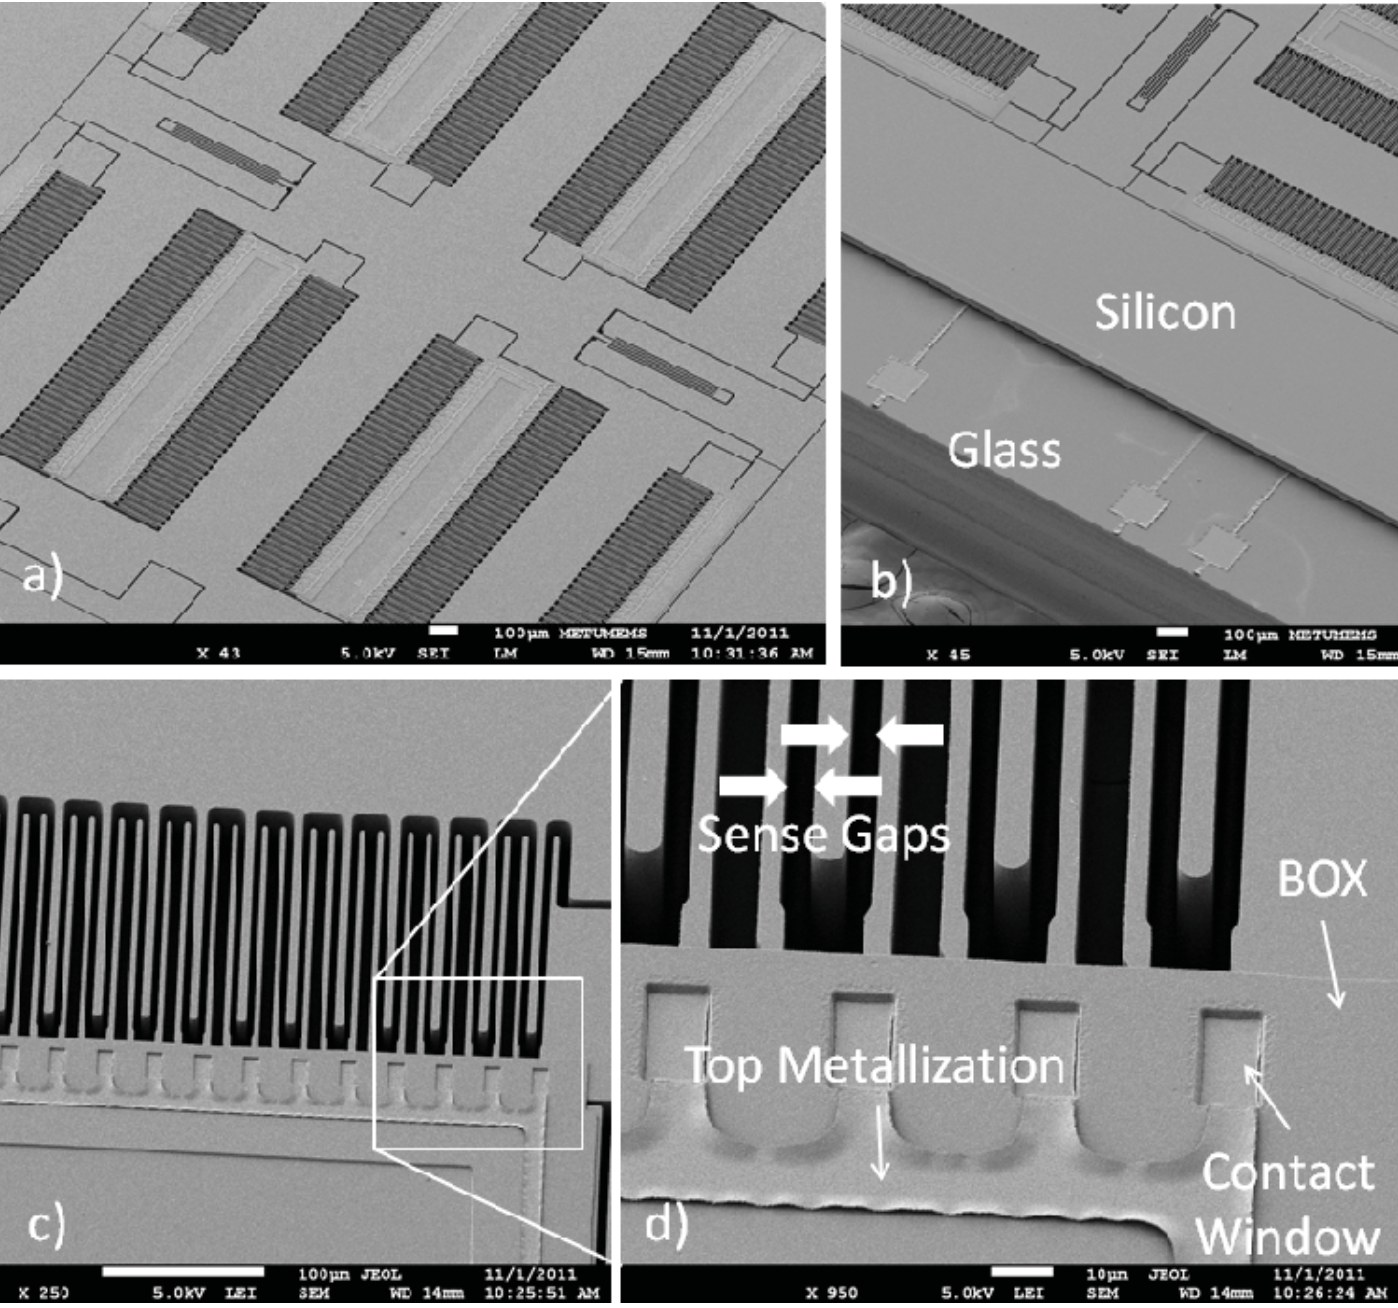
\includegraphics[width = 0.4\textwidth]{images/IMMAGINE_A_1_piastre_inerdigitate .png}
    \caption{Piastre interdigitate}
    \label{fig:etichetta}
\end{figure}

 %%%%%%%%%%%%%%%%% BIBLIOGRAFIA %%%%%%%%%%%%%%%%%
 \begin{thebibliography}{9}
    \bibitem{Manuale1} STMicroelectronics, \emph{rm0433-stm32h742-stm32h743-753-and-stm32h750s REF MANUAL}, [2020].
    \bibitem{Manuale2} Carmine Noviello, \emph{Mastering STM32}, seconda edizione, \emph{Leanpub}, [2022].
    \bibitem{Manuale3} STMicroelectronics, \emph{UM2356-VL53L1X-User\_Manual\_rev1}, [2018].
    \bibitem{Manuale4} InvenSense Inc, \emph{MPU-6000 and MPU-6050 Product Specification}, Revision 3.4, [2013]
    \bibitem{Manulae5} InvenSense Inc, \emph{MPU-6000 and MPU-6050 Register Map and Descriptions}, Revision 4.3, [2013].
    \bibitem{Manuale schematico1} STMicroelectronics, \emph{en.MB1363-H745ZIQ-D01\_Schematic NEW}, [2019].
    \bibitem{Articolo1} Abrami Fabio, \emph{Studio e sviluppo di una piattaforma per il test di droni}, tesi di laurea, relatore: Andrea Bonci, anno accademico [2020-2021].

\end{thebibliography}

\end{document}